% !TeX root = chapter-1-2-3.tex

\selectlanguage{hebrew}

\chapter{הסתברות}

%%%%%%%%%%%%%%%%%%%%%%%%%%%%%%%%%%%%%%%%%%%%%%%%%%%%%%%%%%%%%%%%%%%

\section{קיץ תשע"ח מועד ב}

\begin{center}
\selectlanguage{english}
%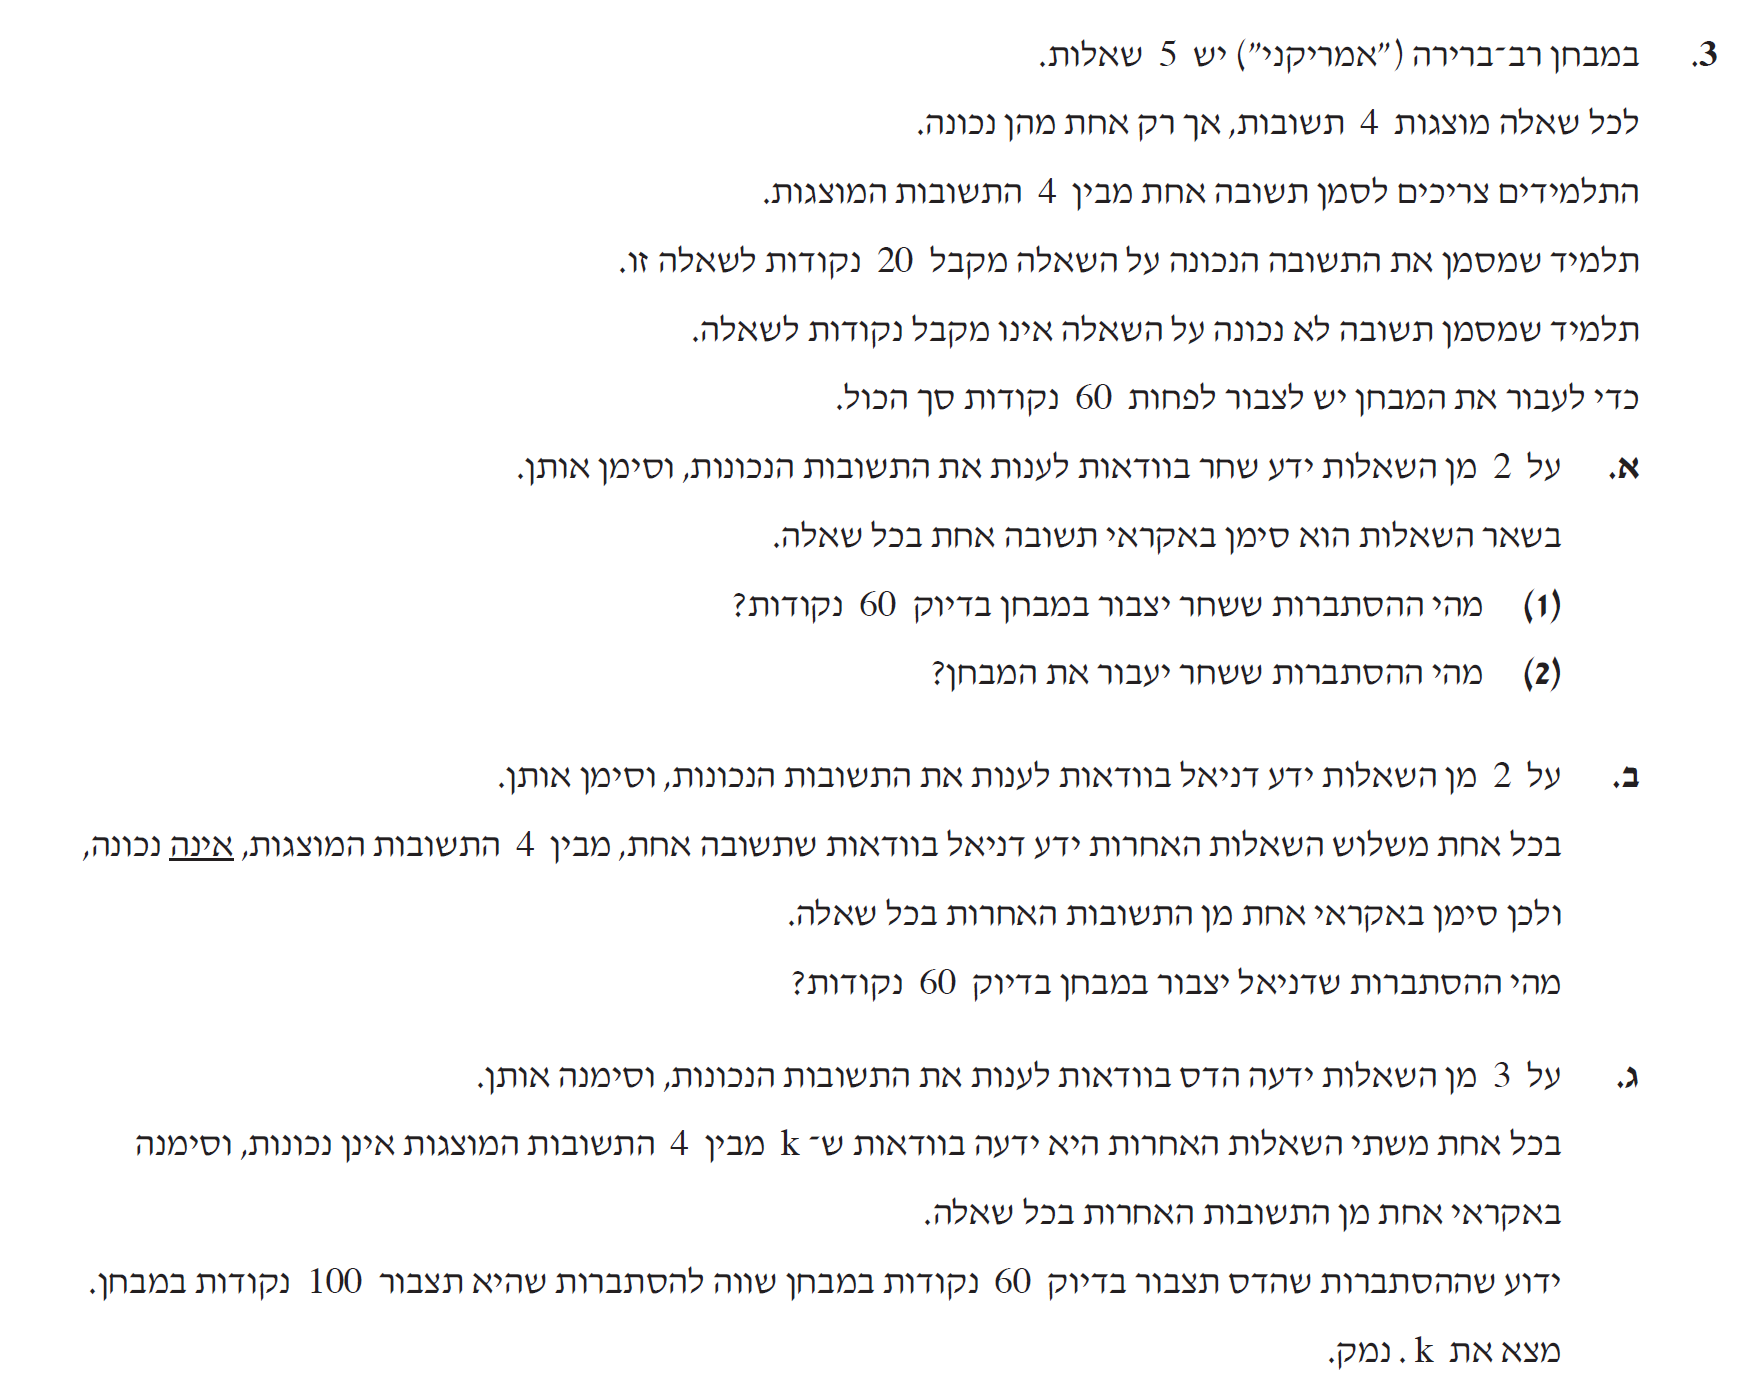
\includegraphics[width=\textwidth]{summer-2018b-3}
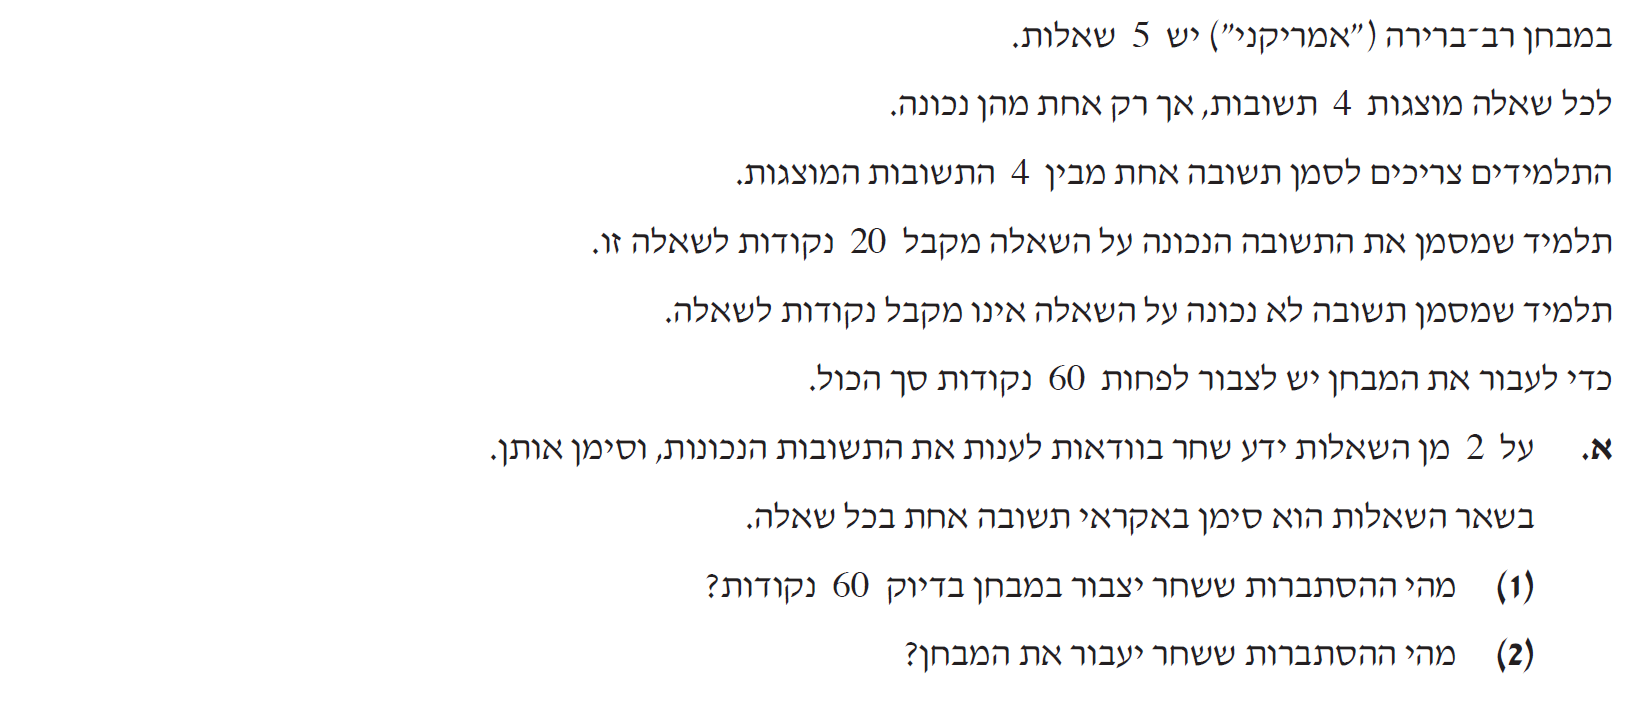
\includegraphics[width=.85\textwidth]{summer-2018b-3-1}
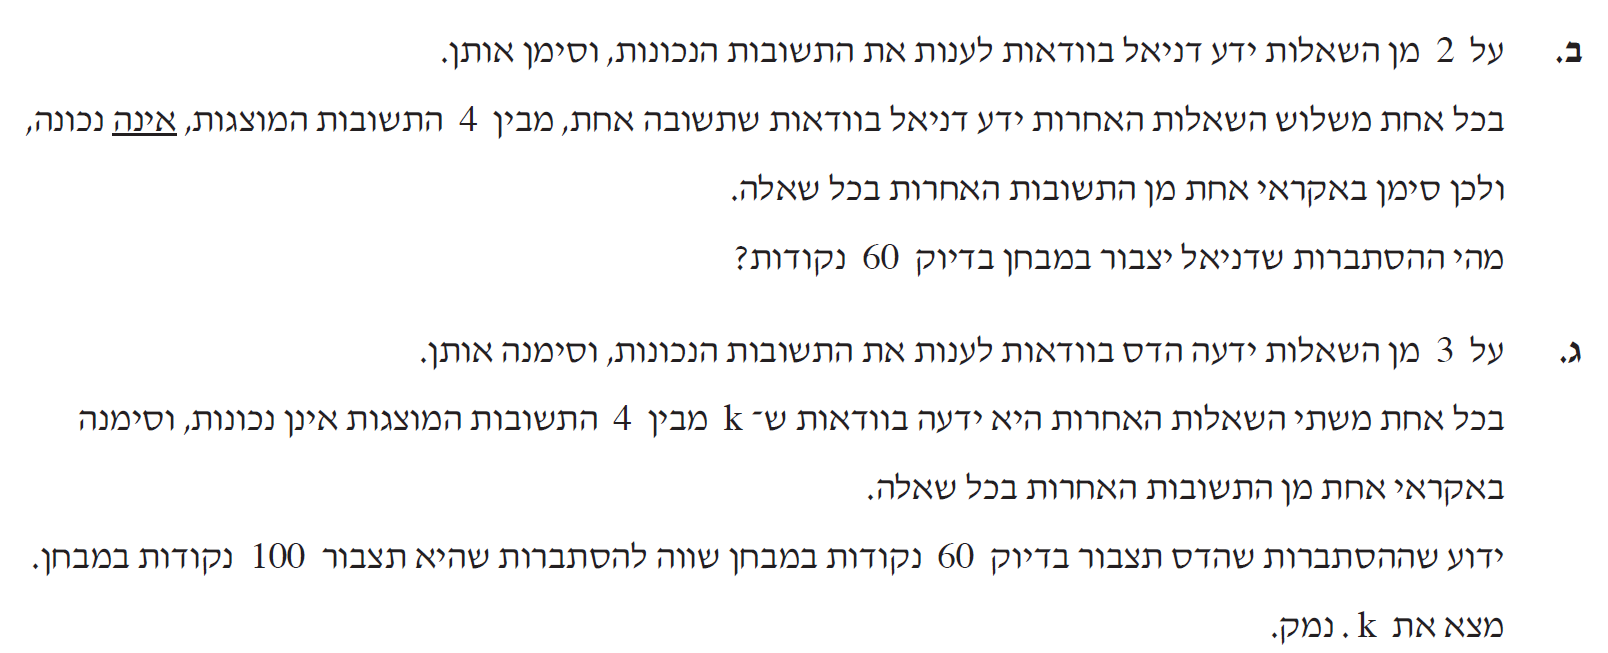
\includegraphics[width=\textwidth]{summer-2018b-3-2}
\end{center}

\textbf{סעיף א}
$(1)$

שחר ידע שהוא ענה נכון על שתי שאלות ולכן כדי לקבל ציון
$60$
עליו לענות על 
\textbf{בדיוק אחת}
משלושת השאלות האחרות:
\[
{3 \choose 1}\left(\frac{1}{4}\right)\left(\frac{3}{4}\right)^2=\frac{27}{64}\,.
\]
\textbf{סעיף א}
$(2)$

כדי לעבור את המבחן עליו לצבור
\textbf{לפחות}
שלוש תשובות נכונות. יש להוסיף את ההסבתרויות של ארבע וחמש תשובות נכונות:
\[
\frac{27}{64}+{3 \choose 2}\left(\frac{1}{4}\right)^2\left(\frac{3}{4}\right)^1+{3 \choose 3}\left(\frac{1}{4}\right)^3\left(\frac{3}{4}\right)^0=\frac{37}{64}\,.
\]
\textbf{סעיף ב}

דניאל צירך לענות נכון על שאלה אחת 
\textbf{בדיוק}
מתוך שלושת השאלות הנותרות. דניאל ידע שתשובה אחת מתוך ארבע לא נכונה, לכן ההסתברות שהוא ענה נכון על השאלה היא
$\frac{1}{3}$:
\[
{3 \choose 1}\left(\frac{1}{3}\right)\left(\frac{2}{3}\right)^2=\frac{4}{9}\,.
\]
\textbf{סעיף ג}

אם הדס ידעה ש-%
$k$
מתוך 
$4$
תשובות לא נכונות, ההסתברות שהיא ענתה תשובה נכונה היא
$\frac{1}{4-k}$,
וההסתברות שהיא תענה תשובה לא נכונה היא
$\frac{4-k-1}{4-k}$.
כדי לקבל ציון 
\textbf{בדיוק}
$100$
הדס צריכה לבחור תשובות נכונות לשתי השאלות הנותרות. כדי לקבל ציון 
\textbf{בדיוק}
$60$
עליה לבחר תשובות לא נכונות לשתי השאלות הנותרות.

אין צורך להשתמש בנוסחת ברנולי במלואו, כי כאשר מחשבים את ההסתברות של "כל" או "אף אחד", 
${n\choose k}=1$,
וגם
$(1-p)^0=1$
או
$p^0=1$.
לכן, מספיק לחשב את ההסתברות של האירוע לחזקת מספר השאלות:
\begin{eqnarray*}
\left(\frac{1}{4-k}\right)^2 &=&\left(\frac{4-k-1}{4-k}\right)^2\\
(3-k)^2&=&1\\
k^2-6k+8&=& 0\,.
\end{eqnarray*}
הפתרונות הם 
$k=2,4$
אבל נתון ש-"אחת ]מהתשובות[ נכונה", לכן הפתרון היחיד הוא
$k=2$.

%%%%%%%%%%%%%%%%%%%%%%%%%%%%%%%%%%%%%%%%%%%%%%%%%%%%%%%%%%%%%%%%%%%
\np
\section{קיץ תשע"ח מועד א}

\begin{center}
\selectlanguage{english}
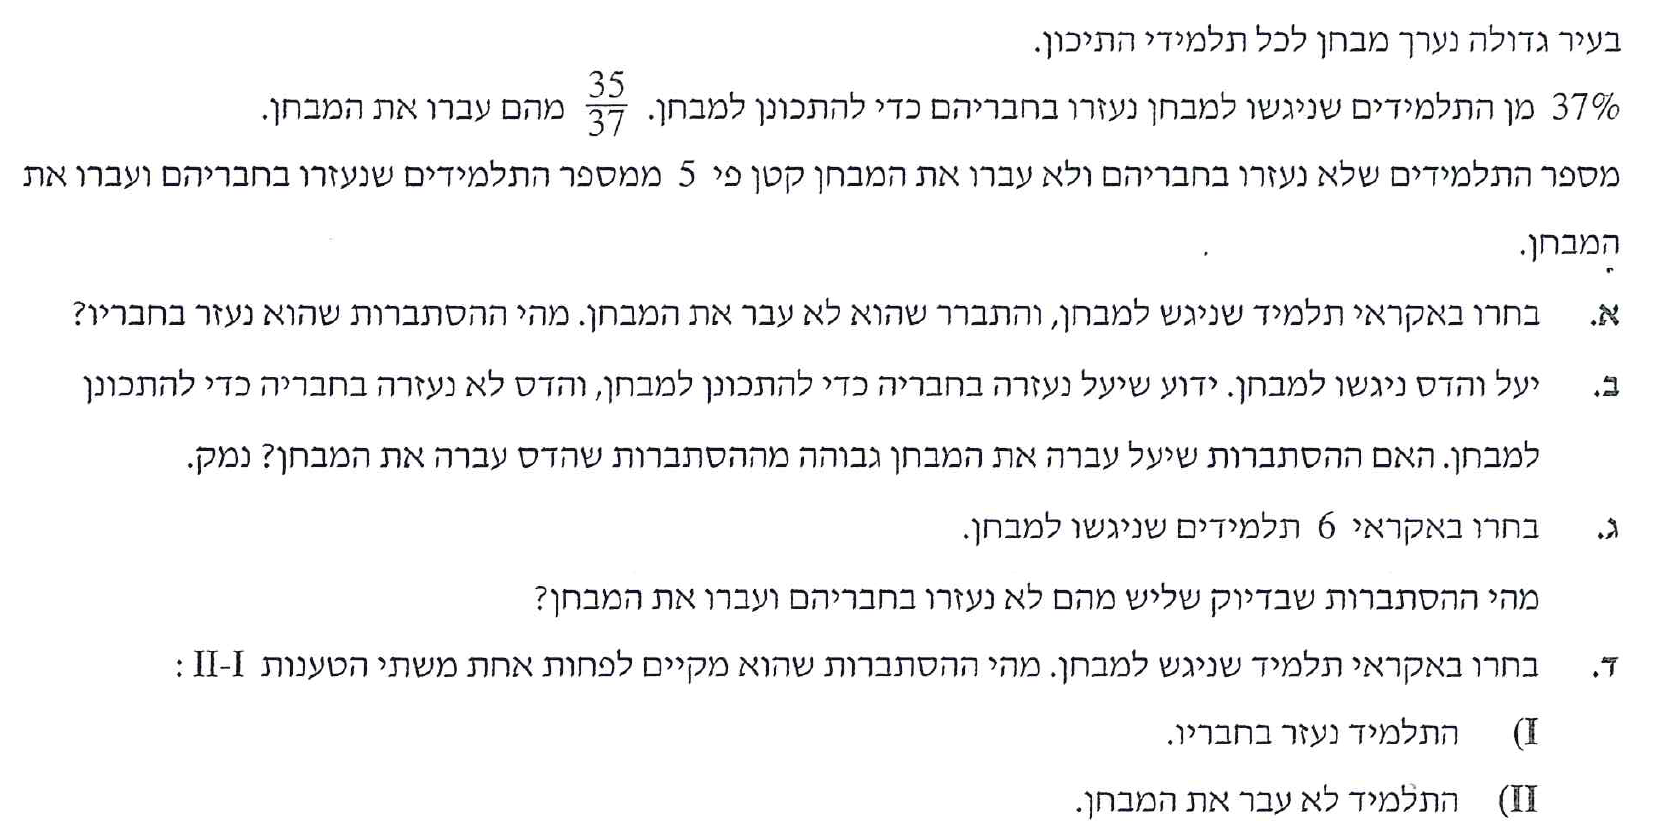
\includegraphics[width=	\textwidth]{summer-2018a-3}
\end{center}
נסמן ב-%
$N$
את התלמידים שנעזרו בחבריהם, וב-%
$A$
את התלמידים שעברו את המבחן. נתון ש-%
$P(N)=0.37$.
\textbf{מהם}
עברו את הבחינה 
$\displaystyle\frac{35}{37}$,
ההסתברות המותנית
$P(A/N)$.
נחשב:
\[
P(A/N) = \frac{P(N\cap A)}{P(N)} = \frac{P(N\cap A)}{0.37}=\frac{35}{37},\quad\quad\quad P(N\cap A)=0.35\,.
\]
עד כאן טבלת ההסתברויות היא:
\begin{center}
\selectlanguage{english}
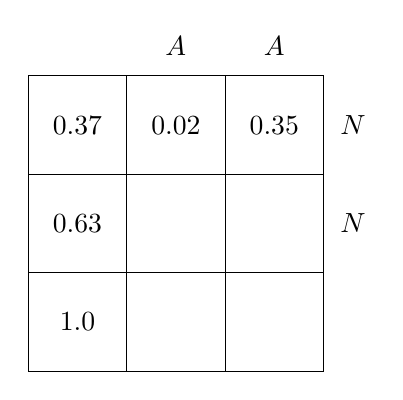
\begin{tikzpicture}[scale=1.25]
\draw (0,0) grid (3,3);
\node at (2.5,3.3) {$\bm{A}$};
\node at (1.5,3.3) {$\bover{A}$};
\node at (3.3,2.5) {$\bm{N}$};
\node at (3.3,1.5) {$\bover{N}$};
\node at (2.5,2.5) {$0.35$};
\node at (0.5,2.5) {$0.37$};
\node at (1.5,2.5) {$0.02$};
\node at (0.5,1.5) {$0.63$};
\node at (0.5,0.5) {$1.0$};
\end{tikzpicture}
\end{center}
בהמשך נתון ש-%
\[
P(\overline{N}\cap\overline{A})=\frac{P(N\cap A)}{5}=\frac{0.35}{5}=0.07\,,
\]
וניתן להשלים את הטבלה:
\begin{center}
\selectlanguage{english}
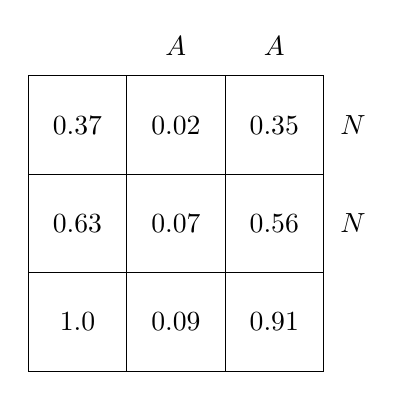
\begin{tikzpicture}[scale=1.25]
\draw (0,0) grid (3,3);
\node at (2.5,3.3) {$\bm{A}$};
\node at (1.5,3.3) {$\bover{A}$};
\node at (3.3,2.5) {$\bm{N}$};
\node at (3.3,1.5) {$\bover{N}$};
\node at (2.5,2.5) {$0.35$};
\node at (0.5,2.5) {$0.37$};
\node at (1.5,2.5) {$0.02$};
\node at (0.5,1.5) {$0.63$};
\node at (0.5,0.5) {$1.0$};
\node at (1.5,0.5) {$0.09$};
\node at (2.5,0.5) {$0.91$};
\node at (1.5,1.5) {$0.07$};
\node at (2.5,1.5) {$0.56$};
\end{tikzpicture}
\end{center}
\textbf{סעיף א}
\[
P(N/\overline{A})=\frac{P(N\cap \overline{A})}{P(\overline{A})}=\frac{0.02}{0.09}=\frac{2}{9}\,.
\]
\textbf{סעיף ב}

עבור יעל:
\[
P(A/N)=\frac{P(A \cap N)}{P(N)}=\frac{0.35}{0.37}=0.9459\,,
\]
ועבור הדס:
\[
P(A/\overline{N})=\frac{P(A\cap \overline{N})}{P(\overline{N})}=\frac{0.56}{0.63}=0.8889\,.
\]
ליעל הסתברות גבוהה יותר לעבור את המבחן.

\textbf{סעיף ג}

שליש של שש הוא שניים. )שימו לב שלא לקרוא "שלושה" במקום "שליש"!( החישוב הוא לפי נוסחת ברנולי כאשר הערך של
$P(\overline{N}\cap A)$
נמצא בטבלה:
\[
{6 \choose 2}(0.56)^2 (1-0.56)^4=0.1763\,.
\]
\textbf{סעיף ד}

הניסוח "%
\textbf{לפחות אחת}
משתי הטענות
$I, II$"
אומר שהאירוע קורה אם קורה אחד מהאירועים
$I, II$
\textbf{או שניהם}.
באיור להלן שני עגולים המייצגים את שני האירועים
$I, II$.
האירוע "לפחות אחד משניהם" מיוצג על ידי כל השטח המקווקו.
\begin{center}
\selectlanguage{english}
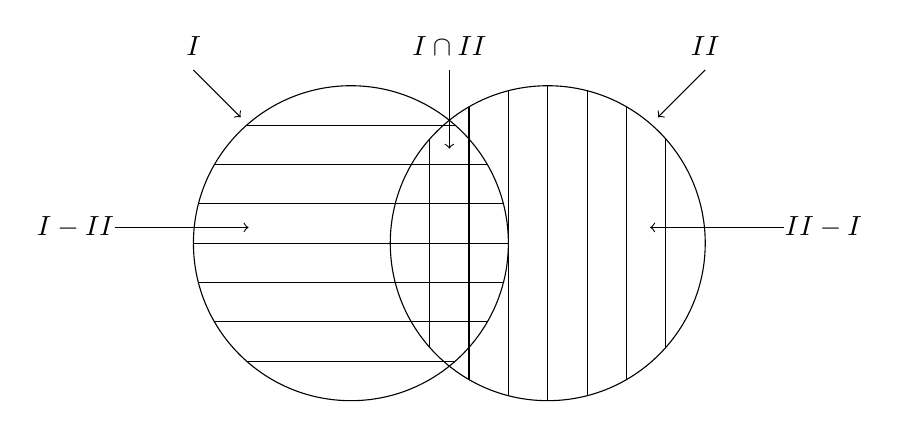
\begin{tikzpicture}
\begin{scope}
\clip[draw] (0,0) circle[radius=2];
\foreach \y in {-1.5,-1,-.5,0,.5,1,1.5}
  \draw (-2,\y) -- (2,\y);
\end{scope}
\begin{scope}
\clip[draw] (2.5,0) circle[radius=2];
\foreach \x in {1,1.5,2,2.5,3,3.5,4}
  \draw (\x,-2) -- (\x,2);
\end{scope}
\node at (-2,2.5) {$I$};
\node at (4.5,2.5) {$II$};
\node at (1.25,2.5) {$I\cap II$};
\node at (-3.5,.2) {$I-II$};
\node at (6,.2) {$II-I$};
\draw[->] (1.25,2.2) -- ++(0,-1);
\draw[->] (-3,.2) -- ++(1.7,0);
\draw[->] (5.5,.2) -- ++(-1.7,0);
\draw[->] (-2,2.2) -- +(.6,-.6);
\draw[->] (4.5,2.2) -- +(-.6,-.6);
\end{tikzpicture}
\end{center}
יש שתי דרכים לחשב את ההסתברות. בדרך הראשונה אנו לוקחים את סכום ההסתברויות של שני האירועים, וחסירים את ההסתברות של האירוע המשותף כי ספרנו אותו פעמיים, פעם כחלק מהאירוע 
$I$
ופעם כחלק מהאירוע
$II$:
\[
P(I \cup II) = P(I) + P(II) - P(I \cap II)\,.
\]
בדרך השניה אנו סופרים כל חלק מהאירוע השותף בנפרד, כאשר הסימון
$A-B$
הוא כל האיברים בקבוצה 
$A$
שאינם בקבוצה
$B$:
\[
P(I \cup II) = P(I-II) + P(II-I) + P(I \cap II)\,.
\]
את ההסתברויות לחישוב ניקח מהטבלה. הדרך הראשונה מופיעה מימין והדרך השניה משמאל:
\begin{center}
\selectlanguage{english}
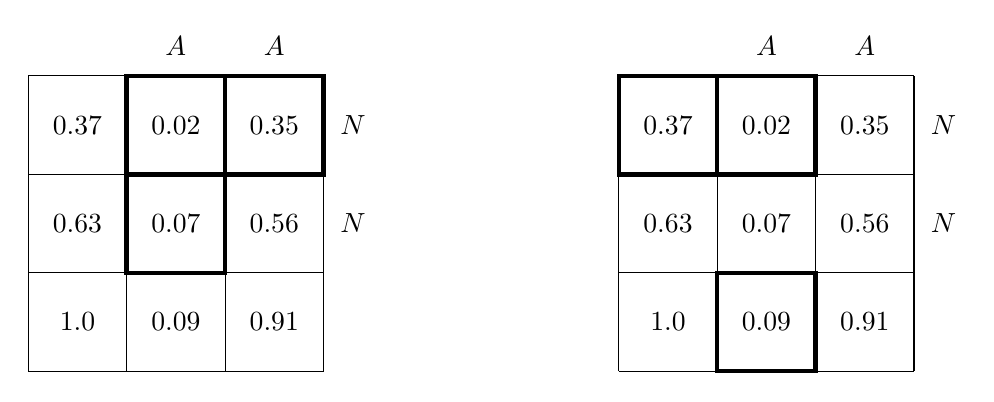
\begin{tikzpicture}[scale=1.25]
\begin{scope}
\draw (0,0) grid (3,3);
\node at (2.5,3.3) {$\bm{A}$};
\node at (1.5,3.3) {$\bover{A}$};
\node at (3.3,2.5) {$\bm{N}$};
\node at (3.3,1.5) {$\bover{N}$};
\node at (2.5,2.5) {$0.35$};
\node at (0.5,2.5) {$0.37$};
\node at (1.5,2.5) {$0.02$};
\node at (0.5,1.5) {$0.63$};
\node at (0.5,0.5) {$1.0$};
\node at (1.5,0.5) {$0.09$};
\node at (2.5,0.5) {$0.91$};
\node at (1.5,1.5) {$0.07$};
\node at (2.5,1.5) {$0.56$};
\draw[ultra thick] (2,2) rectangle +(1,1);
\draw[ultra thick] (1,1) rectangle +(1,1);
\draw[ultra thick] (1,2) rectangle +(1,1);
\end{scope}
\begin{scope}[xshift=6cm]
\draw (0,0) grid (3,3);
\node at (2.5,3.3) {$\bm{A}$};
\node at (1.5,3.3) {$\bover{A}$};
\node at (3.3,2.5) {$\bm{N}$};
\node at (3.3,1.5) {$\bover{N}$};
\node at (2.5,2.5) {$0.35$};
\node at (0.5,2.5) {$0.37$};
\node at (1.5,2.5) {$0.02$};
\node at (0.5,1.5) {$0.63$};
\node at (0.5,0.5) {$1.0$};
\node at (1.5,0.5) {$0.09$};
\node at (2.5,0.5) {$0.91$};
\node at (1.5,1.5) {$0.07$};
\node at (2.5,1.5) {$0.56$};
\draw[ultra thick] (0,2) rectangle +(1,1);
\draw[ultra thick] (1,0) rectangle +(1,1);
\draw[ultra thick] (1,2) rectangle +(1,1);
\end{scope}
\end{tikzpicture}
\end{center}
בשתי הדרכים מקבלים אותה תוצאה:
\[
\renewcommand{\arraystretch}{1.5}
\begin{array}{l}
P(N\cup\overline{A})=P(N) + P(\overline{A}) - P(N\cap\overline{A}) = 0.37+0.09-0.02=0.44\\
P(N\cup\overline{A})=P(N-\overline{A}) + P(\overline{A}-N) + P(N\cap\overline{A}) = 0.35+0.07+0.02=0.44\,.
\end{array}
\]

%%%%%%%%%%%%%%%%%%%%%%%%%%%%%%%%%%%%%%%%%%%%%%%%%%%%%%%%%%%%%%%%%%%

\np
\section{חורף תשע"ח}

\begin{center}
\selectlanguage{english}
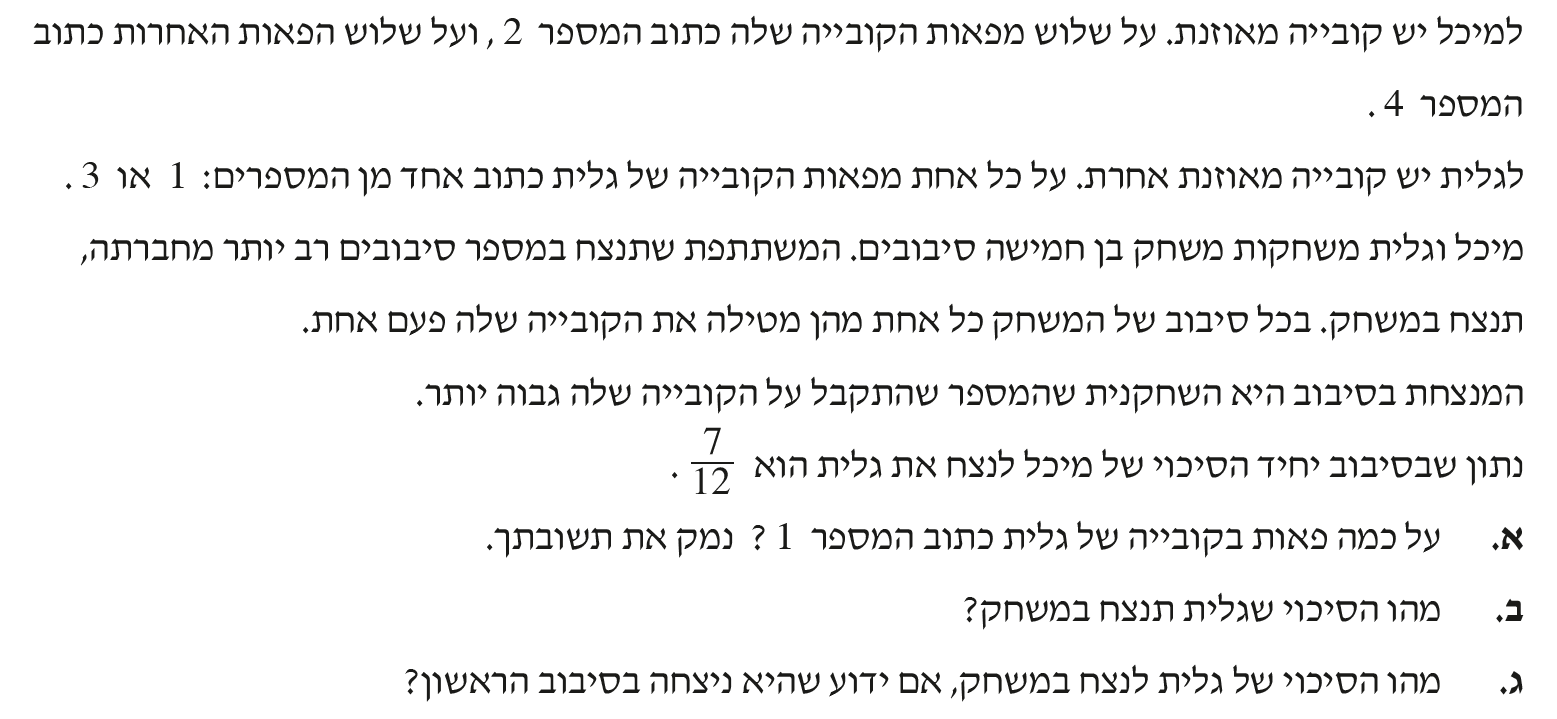
\includegraphics[width=\textwidth]{winter-2018-3}
\end{center}

\textbf{סעיף א}

מיכל תנצח אם )א( היא מטילה 
$4$
לא משנה מה גלית מטילה, אירוע שההסתברות שלה היא 
$1$,
או )ב( מיכל מטילה 
$2$
וגלית מטילה
$1$,
אירוע שההסתברות שלה היא
$\frac{n}{6}$,
כאשר נסמן ב-%
$n$
את המספר הפאות של הקוביה של גלית שכתוב עליהן
$1$.
המשוואה לניצחון של מיכל היא:
\[
\frac{3}{6}\cdot 1 + \frac{3}{6}\cdot \frac{n}{6}=\frac{7}{12}\,,
\]
והפתרון הוא
$n=1$.

\textbf{סעיף ב}

גלית תנצח במשחק אם היא תנצח ב-%
$3,4,5$
סיבובים:
\[
{5\choose 3}\left(\frac{5}{12}\right)^3\left(\frac{7}{12}\right)^2+{5\choose 4}\left(\frac{5}{12}\right)^4\left(\frac{7}{12}\right)^1+{5\choose 5}\left(\frac{5}{12}\right)^5\left(\frac{7}{12}\right)^0=0.3466\,.
\]
\textbf{סעיף ג}

המילים 
\textbf{אם ידוע}
מכוונות להסתברות מותנית:
\vspace{-4ex}
\[
\renewcommand{\arraystretch}{2.4}
\begin{array}{c}
P(\textrm{\R{גלית תנצח}}/\textrm{\R{גלית ניצחה בסיבוב הראשון}}) =\\
\displaystyle\frac{P(\textrm{\R{גלית תנצח}}\cap\textrm{\R{גלית ניצחה בסיבוב הראשון}})}{P(\textrm{\R{גלית ניצחה בסיבוב הראשון}})}\,.
\end{array}
\]
ההסתברות במנה: כדי שגלית תנצח במשחק וגם בסיבוב הראשון, היא חייבת לנצח בסיבוב הראשון וגם ב-%
$2,3,4$
מהסיבובים הנותרים:
\[
\frac{5}{12}\left[{4 \choose 4}\left(\frac{5}{12}\right)^4 \left(\frac{7}{12}\right)^0+
{4 \choose 3}\left(\frac{5}{12}\right)^3 \left(\frac{7}{12}\right)^1+
{4 \choose 2}\left(\frac{5}{12}\right)^2 \left(\frac{7}{12}\right)^2\right]
=\frac{5}{12}\cdot 0.5534\,.
\]
ההסתברות במכנה היא כמובן 
$\frac{5}{12}$,
ולכן התשובה היא
$0.5534$.


%%%%%%%%%%%%%%%%%%%%%%%%%%%%%%%%%%%%%%%%%%%%%%%%%%%%%%%%%%%%%%%%%%%
\np
\section{קיץ תשע"ז מועד ב}

\begin{center}
\selectlanguage{english}
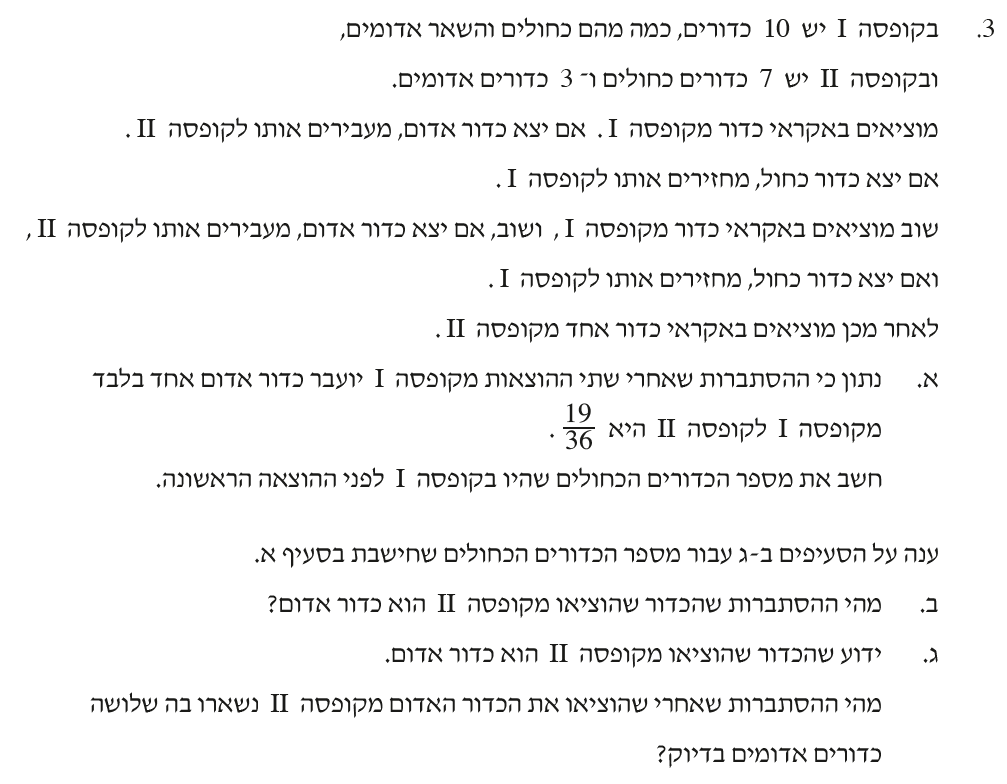
\includegraphics[width=.95\textwidth]{summer-2017b-3}
\end{center}

\vspace{-2ex}

המילים "מוציאים באקראי
$\ldots$
\textbf{ולאחר מכן}
שוב מוציאים באקראי" מכוונות לשימוש בעץ. נסמן ב-%
\textsf{b}
את מספר הכדורים הכחולים בקופסה 
$I$.
באיור~%
\L{\ref{fig.summer-2017b.1}},
בכל צומת רשום שני זוגות של מספרים: מספר הכדורים האדומים ומספר הכדורים הכחולים בקופסה
$I$,
ומתחתיו מספר הכדורים האדומים ומספר הכדורים הכחולים בקופסה
$II$.

\textbf{סעיף א}.

הכוכביות מסמנות את שתי האפשרויות בהן הוצאנו כדור אדום אחד בדיוק מקופסה
\textsf{I}.
\begin{figure}
\begin{center}
\selectlanguage{english}
\begin{tikzpicture}
[grow=right,
level 1/.append style={font=\sffamily,text width=2cm,level distance=5cm,sibling distance=10em},
level 2/.append style={font=\sffamily,text width=2cm,level distance=7cm,sibling distance=6em}]
\node[font=\sffamily,text width=2cm] {(10-b,b)\\(3,7)} % root
child {
  node {(10-b,b)\\(3,7)}
    child {
      node {(10-b,b)\\(3,7)}
      edge from parent node[below] {\R{כחול}}
        node[above,xshift=16mm,yshift=-2mm] {$\frac{b}{10}$}
    }
    child {
      node {(9-b,b)\ *\\(4,7)}
      edge from parent node[above] {\R{אדום}}
        node[below,xshift=16mm,yshift=2mm] {$\frac{10-b}{10}$}
    }
    edge from parent node[below] {\R{כחול}} node[above,xshift=8mm,yshift=0mm] {$\frac{b}{10}$}
}
child { 
  node {(9-b,b)\\(4,7)}
    child {
      node {(9-b,b)\ *\\(4,7)}
      edge from parent node[below] {\R{כחול}}
        node[above,xshift=16mm,yshift=-2mm] {$\frac{b}{9}$}
    }
    child {
      node {(8-b,b)\\(5,7)}
      edge from parent node[above] {\R{אדום}}
        node[below,xshift=16mm,yshift=2mm] {$\frac{9-b}{9}$}
    }
    edge from parent node[above] {\R{אדום}} 
      node[below,xshift=8mm,yshift=0mm] {$\frac{10-b}{10}$}
};
\end{tikzpicture}
\selectlanguage{hebrew}
\setlength{\belowcaptionskip}{-4ex}
\caption{עץ ההסתברויות של הוצאת הכדורים מקופסה $I$}\label{fig.summer-2017b.1}
\end{center}
\end{figure}
נשווה את הסתברות הנתונה לסכום ההסתברויות של שני המסלולים:
\[
\frac{10-b}{10}\cdot\frac{b}{9} + \frac{b}{10}\cdot\frac{10-b}{10} = \frac{19}{36}\,.
\]
נפשט ונקבל משוואה ריבועית 
$b^2-10b+25=0$
שיש לה פתרון אחד
$b=5$.

\textbf{סעיף ב}

לאחר הצבת 
$b=5$,
נקבל עבור כל מצב את מספר הכדורים האדומים וכחולים בקופסה
$II$,
נוכל לחשב את ההסתברויות להוצאת כדור אדום מקופסה
$II$,
ונסכם את ההסתברויות לאחר הכפלתן בהסתברות להגיע לכל אחד מהמצבים:
\[
\renewcommand{\arraystretch}{2}
\begin{array}{l}
\displaystyle\left(\frac{5}{10}\cdot\frac{4}{9}\right)\left(\frac{5}{5+7}\right)+
\left(\frac{5}{10}\cdot\frac{5}{9}\right)\left(\frac{4}{4+7}\right)+\\
\displaystyle\left(\frac{5}{10}\cdot\frac{5}{10}\right)\left(\frac{4}{4+7}\right)+
\left(\frac{5}{10}\cdot\frac{5}{10}\right)\left(\frac{3}{3+7}\right)
=0.3595\,.
\end{array}
\]

\textbf{סעיף ג}

המילים 
"\textbf{ידוע ש-}"
מכוונת להסתברות מותנית:
\vspace{-4ex}
\[
\renewcommand{\arraystretch}{2}
\begin{array}{c}
P(II\ \textrm{\R{נשארו שלושה אדומים בקופסה}}/II\ \textrm{\R{הוציאו כדור אדום מקופסה}}) =\\
\displaystyle\frac{P(II\ \textrm{\R{נשארו שלושה אדומים בקופסה}} \cap II\ \textrm{\R{הוציאו כדור אדום מקופסה}})}{P(II\ \textrm{\R{הוציאו כדור אדום מקופסה}})}
\end{array}
\]
ישארו שלושה כדורים אדומים רק אם היו אברעה כדורים אדומים לפני הבחירה. ההסתברות במנה היא ההסתברות )הנתונה!( שנגיע לאחד המצבים המסומנים בכוכבית כפול ההסתברות לבחור אדום מקופסה 
$II$,
וחישבנו את ההסתברות במכנה בסעיף ב. התשובה היא:
\[
\frac{\displaystyle\frac{19}{36}\cdot\frac{4}{11}}{0.3595}=0.53385\,.
\]

%%%%%%%%%%%%%%%%%%%%%%%%%%%%%%%%%%%%%%%%%%%%%%%%%%%%%%%%%%%%%%%%%%%
\np
\section{קיץ תשע"ז מועד א}

\begin{center}
\selectlanguage{english}
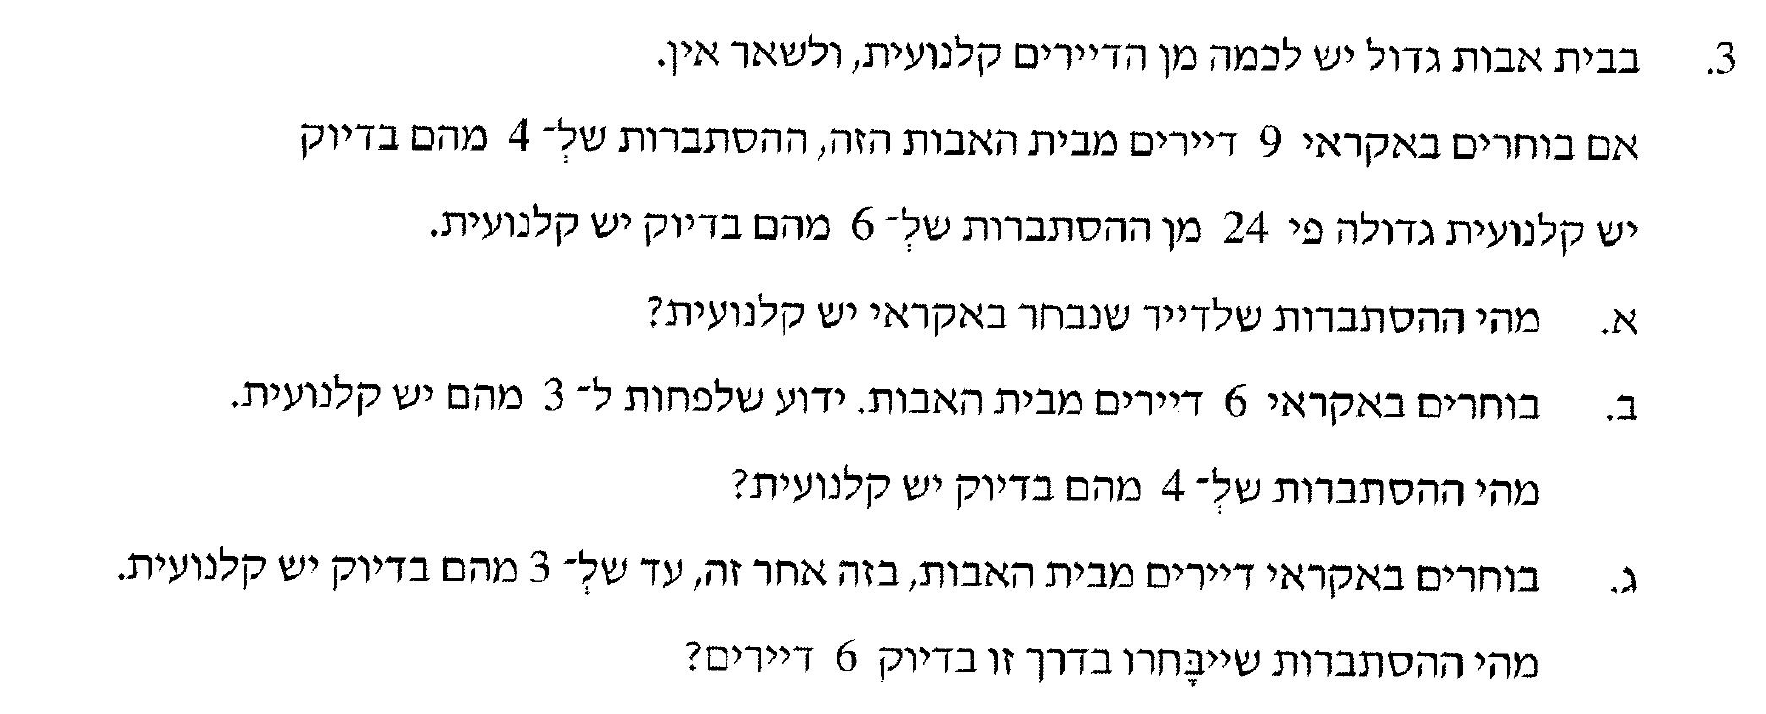
\includegraphics[width=.95\textwidth]{summer-2017a-3}
\end{center}

\textbf{סעיף א}

נסמן ב-%
$D$
את האירוע "לדייר יש קלנועית" ואת ההסתברות של האירוע ב-%
$p$.
נתון ש:
\[
{9\choose 4} p^4 (1-p)^5=24 {9\choose 6} p^6 (1-p)^3\,.
\]
נפשט ונקבל משוואה ריבועית:
\[
15p^2+2p-1=0\,,
\]
עם שני פתרונות
$p=\frac{1}{5},-\frac{1}{3}$.
הסתברות חייבת להיות לא-שלילית ולכן התשובה היא 
$p=\frac{1}{5}=0.2$.

\textbf{סעיף ב}

המילים
"\textbf{ידוע ש-}"
מכוונות להסתברות מותנית:
\[
P(D=4/D\ge3) = \frac{P(D=4\cap D\ge 3)}{P(D\ge 3)}\,.
\]
כאשר יש חפיפה בין שני ביטויים בחיתוך אפשר לפשט אותו. ברור שאם ערך גדול או שווה
$3$
\textbf{וגם}
שווה ל-%
$4$
אז הוא שווה ל-%
$4$:
\[
P(D=4/D\ge3) =\frac{P(D=4)}{P(D\ge 3)}\,.
\]
לפי נוסחת ברנולי:
\[
P(D=4)={6\choose 4} 0.2^4 (1-0.2)^2= 0.01536\,.
\]
את הערך של
$P(D\ge 3)$
אפשר לחשב בשתי דרכים, בצורה ישירה או כאחד פחות המשלים. נבחר את האפשרות השנייה כי יש פחות גורמים בביטוי:
\[
1-0.2^0(1-0.2)^6-{6\choose 1}0.2^1(1-0.2)^5 - {6 \choose 2} 0.2^2(1-0.2)^4=0.099\,,
\]
והתשובה היא
$\displaystyle\frac{0.01536}{0.099}=0.15534$.

\newpage

\textbf{סעיף ג}

הבחירה 
\textbf{האחרונה} 
תהיה "הצלחה" ויהיו שתי "הצלחות" בחמשת הבחירות הקודמות:
\[
\overbrace{\pm\;\pm\;\pm\;\pm\;\pm}^{2/5}\quad\quad \overbrace{+}^{1/1}\,.
\]
התשובה מתקבלת מנוסחת ברנולי לבחירות הראשונות כפול ההסתברות
$p$
לבחירה האחרונה:
\[
\left[{5\choose 2}0.2^2 (1-.02)^3\right]\cdot 0.2=0.04096\,.
\]

%%%%%%%%%%%%%%%%%%%%%%%%%%%%%%%%%%%%%%%%%%%%%%%%%%%%%%%%%%%%%%%%%%%
\np
\section{חורף תשע"ז}

\begin{center}
\selectlanguage{english}
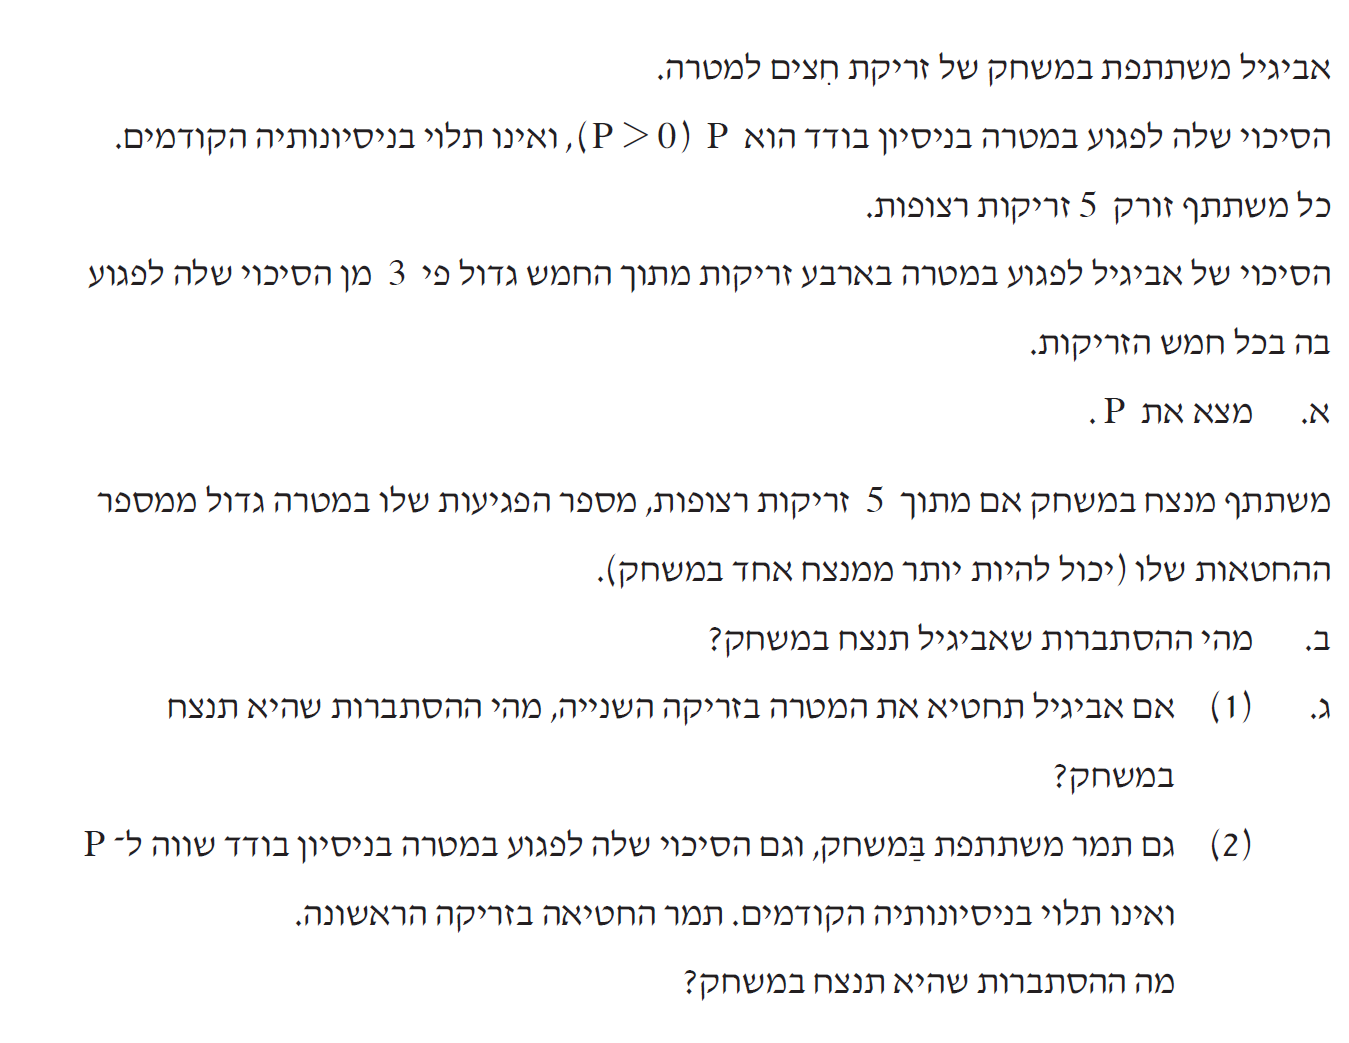
\includegraphics[width=.95\textwidth]{winter-2017-3.png}
\end{center}
\vspace{-1ex}

\textbf{סעיף א}

לפי המידע הנתון:
\[
{5 \choose 4} p^4(1-p)^1 = 3{5\choose 5}p^5(1-p)^0\,.
\]
והפתרון הוא
$p=\frac{5}{8}$.

\textbf{סעיף ב}

ההסתברות ל-%
$3,4,5$
פגיעות היא:
\[
{5 \choose 3}p^3(1-p)^2 + {5 \choose 4}p^4(1-p)^1 + {5 \choose 5}p^5(1-p)^0
\]
נציב
$p=\frac{5}{8}$
ונקבל
$0.7248$.

\textbf{סעיף ג} 
$(1)$

לדעתי, ניסוח השאלה לא ברור. אני פירשתי אותה: מה ההסתברות של
\textbf{האירוע}
"אביגיל מחטיאה בזריקה השנייה ופוגעת בשלוש או ארבע מהזריקות האחרות"? כותב הבחינה התכוון להסתברות מותנית: "%
\textbf{אם ידוע ש-}%
אביגיל החטיאה בזריקה השנייה, מה ההסתברות שהיא פוגעת בשלוש או ארבע מהזריקות האחרות"?
\[
\renewcommand{\arraystretch}{2}
\begin{array}{c}
P(1,3,4,5\ \textrm{\R{אביגיל פגעה בשלוש או ארבע מהזריקות}}/\textrm{\R{אביגיל החטיאה בזריקה השניה}}) =\\
\displaystyle\frac{P(1,3,4,5\ \textrm{\R{אביגיל פגעה בשלוש או ארבע מהזריקות}}\cap \textrm{\R{אביגיל החטיאה בזריקה השניה}})}{P(\textrm{\R{אביגיל החטיאה בזריקה השניה}})}\,.
\end{array}
\]
אפשר לפתור את הבעיה בשתי דרכים. נתחיל עם הדרך הפשוטה יותר. נתון שהסיכוי לפגוע במטרה אינו תלוי בניסיונות הקודמים, ולכן ההסתברויות בלתי תלויות והחישוב מצטמצם:
\[
\renewcommand{\arraystretch}{2}
\begin{array}{c}
\displaystyle\frac{P(1,3,4,5\ \textrm{\R{אביגיל פגעה בשלוש או ארבע מהזריקות}}) \cdot P(\textrm{\R{אביגיל החטיאה בזריקה השניה}})}{P(\textrm{\R{אביגיל החטיאה בזריקה השניה}})}=\\
P(1,3,4,5\ \textrm{\R{אביגיל פגעה בשלוש או ארבע מהזריקות}})\,.
\end{array}
\]
החישוב הוא:
\[
{4\choose 4}\left(\frac{5}{8}\right)^4 \left(\frac{3}{6}\right)^0 +{4\choose 3}\left(\frac{5}{8}\right)^3\left(\frac{3}{8}\right)^1 = 0.5188\,.
\]
הדרך השנייה ארוכה יותר אבל מעניינת. האירוע של החיתוך בנוסחה להסתברות מותנית מורכבת משני אירועים: )א( לא משנה מה יצאה מהזריקה הראשונה, הזריקה השניה החטיאה, ושלושת הזריקות האחרונות פגעו. )ב( הזריקה הראשונה פגעה, הזריקה השניה החטיאה, ושתיים מתוך שלושת הזריקות האחרונות פגעו. הסתברות של האירוע המשותף היא:
\[
1\cdot \frac{3}{8} \cdot \left(\frac{5}{8}\right)^3 \quad + \quad
\frac{5}{8}\cdot \frac{3}{8} \cdot \left[{3\choose 2}\left(\frac{5}{8}\right)^2\frac{3}{8}\right] = 0.1945\,.
\]
נחלק ב-%
$\frac{3}{8}$,
ההסתברות האביגיל החטיאה בזריקה השנייה, ונקבל 
$0.5188$.

\textbf{סעיף ג} 
$(2)$

לא משנה איזו זריקה החטיאה, הזריקות בלתי תלויות וחישוב ההסתברות של "תמר פגעה בשלוש  או ארבע מהזריקות 
$2,3,4,5$"
נותן אותה תוצאה כמו האירוע "אביגיל פגעה בשלוש או ארבע מהזריקות 
$1,3,4,5$".

%%%%%%%%%%%%%%%%%%%%%%%%%%%%%%%%%%%%%%%%%%%%%%%%%%%%%%%%%%%%%%%%%%%
\np
\section{קיץ תשע"ו מועד ב}

\begin{center}
\selectlanguage{english}
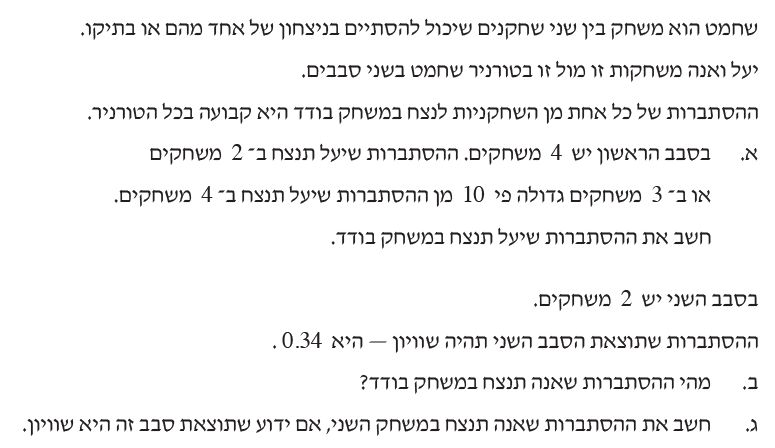
\includegraphics[width=.86\textwidth]{summer-2016b-3}
\end{center}

\vspace{-2ex}

נסמן:
$=y$
ההסתברות שיעל תנצח במשחק בודד, 
$=a$
ההסתברות שאנה תנצח במשחק בודד.

\textbf{סעיף א}

לפי המידע הנתון:
\[
{4 \choose 2}y^2(1-y)^2 + {4\choose 3}y^3(1-y) = 10\cdot {4\choose 4}y^4(1-y)^0\,.
\]
נפשט ונקבל משוואה ריבועית
$4y^2+4y-3=0$
שהשורש החיובי היחיד שלה היא
$y=\frac{1}{2}$.

\textbf{סעיף ב}

כדאי לצייר עץ של האירועים, אבל אוותר עליו בשאלה זו כי המצב פשוט. האפשרויות לקבל שוויון הן: )א( ניצחון אחד לאנה וליעל, או )ב( תיקן בשני המשחקים. ההסתברות לתיקו היא המשלים לסכום ההסתברויות שאחת מהן תנצח:
\[
{2 \choose 1}ya + (1-(y+a))^2 = 0.34\,.
\]
נציב 
$y=\frac{1}{2}$
ונקבל
$a=0.3$.

\textbf{סעיף ג}

המילים
"\textbf{אם ידוע ש-}"
מכוונות להסתברות מותנית:
\vspace{-2ex}
\[
\renewcommand{\arraystretch}{2}
\begin{array}{c}
P(\textrm{\R{אנה תנצח במשחק השני}} / \textrm{\R{תוצאת הסבב השני היא שוויון}})=\\
\displaystyle\frac{
P(\textrm{\R{אנה תנצח במשחק השני}} \cap \textrm{\R{תוצאת הסבב השני היא שוויון}})
}
{P(\textrm{\R{תוצאת הסבב השני היא שוויון}})}\,.
\end{array}
\]
ההסתברות לשיוון בסבב השני נתונה. אם אנה תנצח במשחק השני, יהיה שוויון רק אם גם יעל תנצח במשחק הראשון:
\vspace{-1ex}
\[
\frac{ya}{.34}=\frac{\displaystyle\frac{1}{2}\cdot 0.3}{.34}=0.4412\,.
\]
שימו לב שלא צריכים
$2 \choose 1$
כי האירוע הוא שאנה תנצח במשחק 
\textbf{השני}
ויעל תנצח במשחק
\textbf{הראשון}.

%%%%%%%%%%%%%%%%%%%%%%%%%%%%%%%%%%%%%%%%%%%%%%%%%%%%%%%%%%%%%%%%%%%
\np
\section{קיץ תשע"ו מועד א}

\begin{center}
\selectlanguage{english}
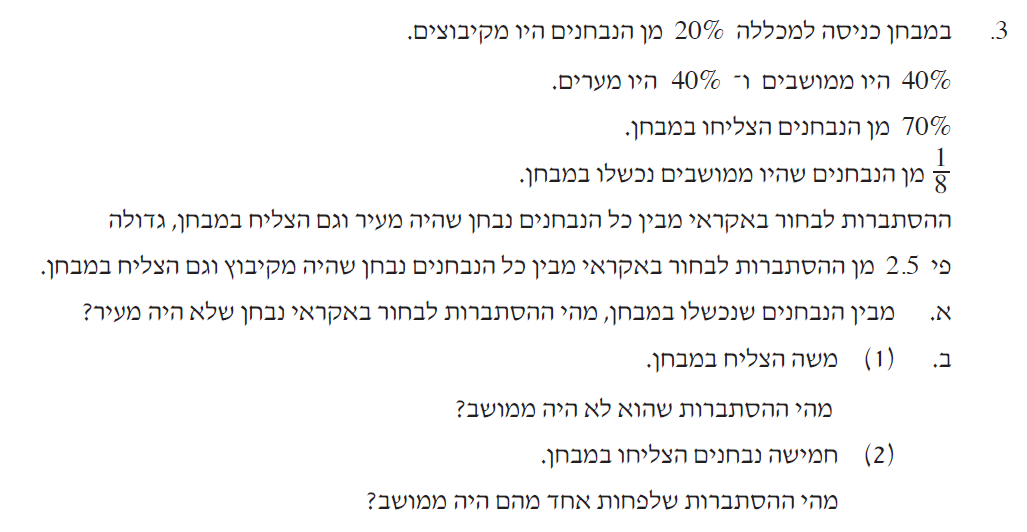
\includegraphics[width=.95\textwidth]{summer-2016a-3}
\end{center}

נסמן 
$=S$
נבחנים שהצליחו,
$=K$
נבחנים מקיבוצים,
$=M$
נבחנים ממושבים,
$=E$
נבחנים מערים. ההסתברויות הנתונות הן:
\[
P(K)=0.20,\;P(M)=0.40,\;P(E)=0.40,\;P(S)=0.70\,.
\]
נחשב את שאר ההסתברויות. לפי הסתברות משלימה
$P(\overline{S})=1-P(S)=0.30$.
נתון:
\[
P(\overline{S}/M)=P(\overline{S}\cap M) / P(M)=\frac{1}{8}\,,
\]
ולכן:
\[
P(\overline{S}\cap M)=\frac{1}{8}P(M)=0.05\,.
\]
לפי ההגדרה:
\[
P(S)=P(K\cap S) + P(M\cap S) + P(E\cap S)\,.
\]
נסמן
$P(K\cap S)=p$,
ההסתברות שנבחנים מקיבוצים הצליחו. נתון:
\[
P(E\cap S)=2.5P(K\cap S)=2.5p\,,
\]
ולכן:
\[
0.70=p+(0.40-0.05)+2.5p\,,
\]
ו-%
$p=0.1$.

שימו לב שהמילים 
"$\frac{1}{8}$
\textbf{מן}
הנבחנים שהיו ממושבים נכשלו" מכוונות להסתברות מותנית, לעומת המילים "ההסתברות לבחור באקראי
\textbf{מבין כל}
הנבחנים נבחן שהיה מהעיר
\textbf{וגם}
הצליח במבחן" מכוונות לחיתוך הסתברויות. המילה "מבין" בדרך כלל מכוונת להסתברות מותנית, אבל כאשר "מבין" מתייחס ל-%
"\textbf{כל}
הנבחנים" אין הסתברות מותנית. לחילופין, ההסתברות לבחור אחד "מכל הנבחנים" היא 
$1$,
ולכן:
\[
P(E\cap S/\textrm{\R{כל הנבחנים}})=
\frac{(P(E\cap S)\cap \textrm{\R{כל הנבחנים}})}
{P(\textrm{\R{כל הנבחנים}})} = 
\frac{P(E\cap S)}{1}=P(E\cap S)\,.
\]
נסכם את המידע בטבלה:
\begin{center}
\selectlanguage{english}
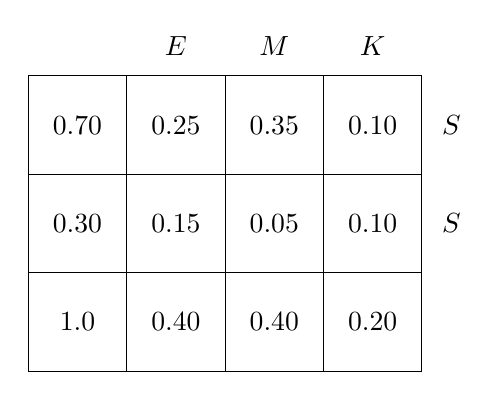
\begin{tikzpicture}[scale=1.25]
\draw (0,0) grid (4,3);
\node at (3.5,3.3) {$\bm{K}$};
\node at (2.5,3.3) {$\bm{M}$};
\node at (1.5,3.3) {$\bm{E}$};
\node at (4.3,2.5) {$\bm{S}$};
\node at (4.3,1.5) {$\bover{S}$};

\node at (0.5,2.5) {$0.70$};
\node at (0.5,1.5) {$0.30$};
\node at (0.5,0.5) {$1.0$};

\node at (1.5,2.5) {$0.25$};
\node at (1.5,1.5) {$0.15$};
\node at (1.5,0.5) {$0.40$};

\node at (2.5,2.5) {$0.35$};
\node at (2.5,1.5) {$0.05$};
\node at (2.5,0.5) {$0.40$};

\node at (3.5,2.5) {$0.10$};
\node at (3.5,1.5) {$0.10$};
\node at (3.5,0.5) {$0.20$};
\end{tikzpicture}
\end{center}
\textbf{סעיף א}

לפי הנוסחה להסתברות מותנית:
\[
P(\overline{E}/\overline{S})=P((K\cup M)/\overline{S}) = \frac{P(K\cap \overline{S})+P(M\cap \overline{S})}{P(\overline{S})}=\frac{0.10+0.05}{0.30}=\frac{1}{2}\,.
\]
\textbf{סעיף ב}
$(1)$

לפי הנוסחה להסתברות מותנית:
\[
P(\overline{M}/S)=P((K\cup E)/S) = \frac{P(K\cap S)+P(E\cap S)}{P(S)}=\frac{0.10+0.25}{0.70}=\frac{1}{2}\,.
\]
\textbf{סעיף ב}
$(2)$

"לפחות אחד ממושב" הוא המשלים ל-"כולם לא מהמושב":
\[
1-P(\overline{M}/S)^5=1-\left(\frac{1}{2}\right)^2=\frac{31}{32}\,.
\]

%%%%%%%%%%%%%%%%%%%%%%%%%%%%%%%%%%%%%%%%%%%%%%%%%%%%%%%%%%%%%%%%%%%
\np
\section{חורף תשע"ו}

\begin{center}
\selectlanguage{english}
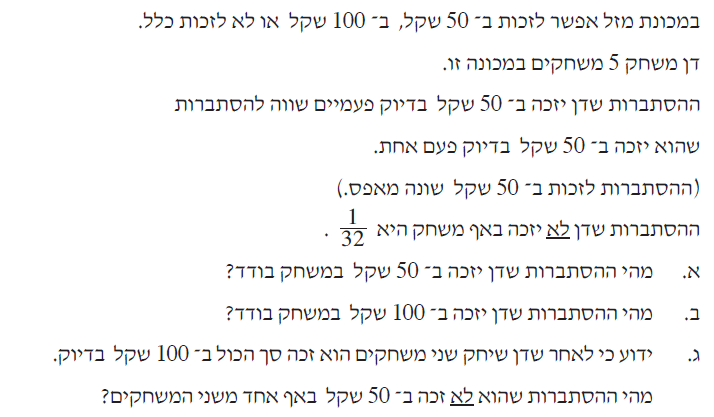
\includegraphics[width=.85\textwidth]{winter-2016-3}
\end{center}
\textbf{סעיף א}

ההסתברות שדן לא יזכה באף אחד מחמישת המשחקים היא 
$P(0)^5$.
נתון שערך זה הוא 
$\frac{1}{32}$,
ולכן 
$P(0)=\frac{1}{2}$.
לפי המידע הנתון:
\begin{eqnarray*}
{5\choose 2} P(50)^2 (1-P(50))^3 &=& {5\choose 1} P(50) (1-P(50))^4\\
P(50)&=&\frac{1}{3}\,.
\end{eqnarray*}
\textbf{סעיף ב}

לפי ההסתברות המשלימה:
$\displaystyle P(100) = 1 - P(0) - P(50) = 1-\frac{1}{2}-\frac{1}{3}=\frac{1}{6}$.

\textbf{סעיף ג}

המילים
"\textbf{ידוע כי}"
מכוונות להסתברות מותנית:
\vspace{-4ex}
\[
\renewcommand{\arraystretch}{2}
\begin{array}{c}
P(\textrm{\R{ באף משחק}}50\textrm{\R{לא זכה ב-}}
/
\textrm{\R{ בשני משחקים}}
100\textrm{\R{זכה ב-}}) =\\
\displaystyle\frac{
P(\textrm{\R{ באף משחק}}50\textrm{\R{לא זכה ב-}}
\cap
\textrm{\R{ בשני משחקים}}
100\textrm{\R{זכה ב-}})
}
{P(
\textrm{\R{ בשני משחקים}}
100\textrm{\R{זכה ב-}})}\,.
\end{array}
\]
נתבונן בעץ המציג את תוצאות שני המשחקים )איור~%
\L{\ref{fig.winter-2017.1}}(.
סימנו את המסלולים שבהם דן זכה ב-%
$100$
והמסלולים בהם דן לא זכה ב-%
$50$
באף אחד משני המשחקים.
\begin{figure}
\begin{center}
\selectlanguage{english}
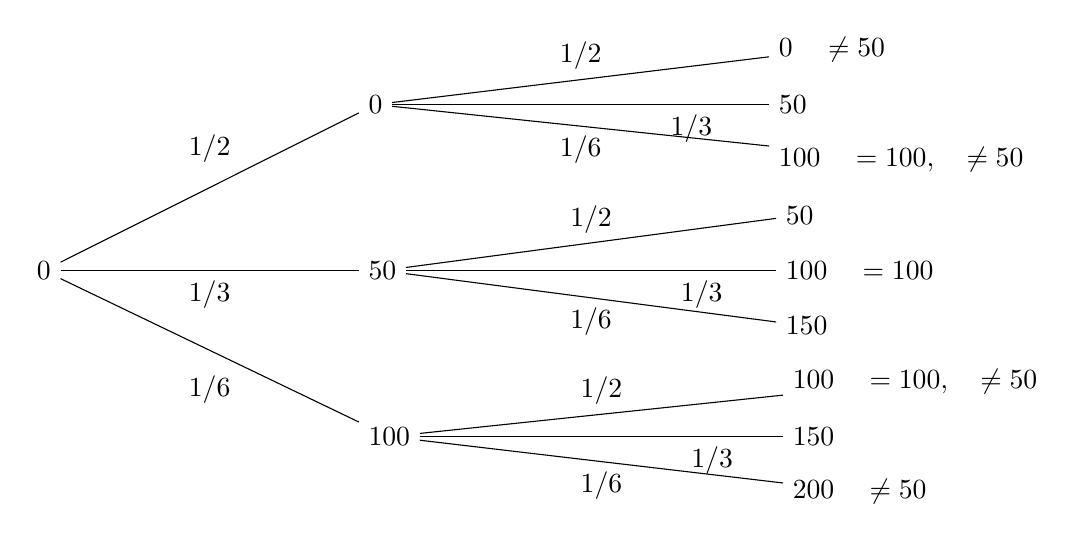
\begin{tikzpicture}
[grow=right,
level 1/.append style={font=\sffamily,level distance=4cm,sibling distance=6em},
level 2/.append style={font=\sffamily,level distance=5cm,sibling distance=2em}]
\node[left] {$0$} % root
child {
  node[right] {$100$}
    child {
      node[right] {$200\quad \neq 50$}
      edge from parent node[below] {$1/6$}
    }
    child {
      node[right] {$150$}
      edge from parent node[below,xshift=4em] {$1/3$}
    }
    child {
      node[right] {$100\quad =100,\quad \neq 50$}
      edge from parent node[above] {$1/2$}
    }
    edge from parent node[below,yshift=-2mm] {$1/6$}
}
child {
  node[right] {$50$}
    child {
      node[right] {$150$}
      edge from parent node[below] {$1/6$}
    }
    child {
      node[right] {$100\quad =100$}
      edge from parent node[below,xshift=4em] {$1/3$}
    }
    child {
      node[right] {$50$}
      edge from parent node[above] {$1/2$}
    }
    edge from parent node[below] {$1/3$}
}
child {
  node[right] {$0$}
    child {
      node[right] {$100\quad =100,\quad \neq 50$}
      edge from parent node[below] {$1/6$}
    }
    child {
      node[right] {$50$}
      edge from parent node[below,xshift=4em] {$1/3$}
    }
    child {
      node[right] {$0\quad \neq 50$}
      edge from parent node[above] {$1/2$}
    }
    edge from parent node[above,yshift=2mm] {$1/2$}
}
;
\end{tikzpicture}
\selectlanguage{hebrew}
\setlength{\belowcaptionskip}{-6ex}
\caption{עץ ההסתברויות של המשחקים}\label{fig.winter-2017.1}
\end{center}
\end{figure}
חישוב ההסתברות המותנית:
\[
\frac{\displaystyle\frac{1}{2}\cdot\frac{1}{6} + \frac{1}{6}\cdot \frac{1}{2}}{\displaystyle\frac{1}{2}\cdot\frac{1}{6} + \frac{1}{3}\cdot \frac{1}{3}+ \frac{1}{6}\cdot \frac{1}{2}}  =  \frac{\displaystyle\frac{1}{6}}{\displaystyle\frac{5}{18}}=\frac{3}{5}\,.
\]

%%%%%%%%%%%%%%%%%%%%%%%%%%%%%%%%%%%%%%%%%%%%%%%%%%%%%%%%%%%%%%%%%%%
\np
\mbox{}
\np

\section{קיץ תשע"ה מועד ב}

\begin{center}
\selectlanguage{english}
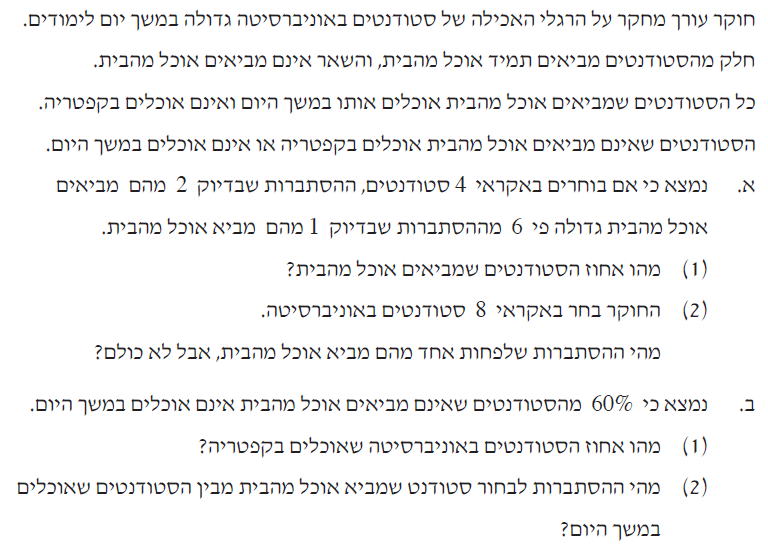
\includegraphics[width=.85\textwidth]{summer-2015b-3}
\end{center}

\vspace{-2ex}

\textbf{סעיף א}
$(1)$

נסמן
$=b$
ההסתברות להביא אוכל מהבית. לפי המידע הנתון:
\[
{4 \choose 2} b^2(1-b)^2 = 6\cdot {4 \choose 1} b (1-b)^3\,.
\]
פתרון המשוואה הוא 
$b=\frac{4}{5}$.

\textbf{סעיף א}
$(2)$

"לפחות אחד אבל לא כולם" היא המשלים ל-"לא אפס ולא כולם":
\[
1-\left(\frac{1}{5}\right)^8-\left(\frac{4}{5}\right)^8=0.8322\,.
\]
\textbf{סעיף ב}
$(1)$

בעץ ההסתברויות באיור~%
\L{\ref{fig.summer-2015b.1}}
הכוכבית מראה את מהמסלול עבור "אוכל בקפטריה":
\[
\frac{1}{5}\cdot \frac{4}{10} = \frac{2}{25}\,.
\]
\textbf{סעיף ב}
$(2)$

המילה
"\textbf{מבין}"
מכוונת להסתברות מותנית, כאשר קבוצת "מביא אוכל" היא תת-קבוצה של "אוכלים" והחישוב מצטמטם:
\[
%\vspace{-1ex}
\renewcommand{\arraystretch}{2}
\begin{array}{c}
P(\textrm{\R{מביא אוכל}} / \textrm{\R{אוכלים}})=\\
\displaystyle\frac{
P(\textrm{\R{מביא אוכל}} \cap \textrm{\R{אוכלים}})
}
{P(\textrm{\R{אוכלים}})}=\\
\displaystyle\frac{
P(\textrm{\R{מביא אוכל}})
}
{P(\textrm{\R{אוכלים}})}\,.
\end{array}
\]
החישוב הוא:
\[
\frac{4/5}{\displaystyle\frac{4}{5}+\frac{2}{25}}=\frac{10}{11}\,.
\]

\begin{figure}[H]
\begin{center}
\selectlanguage{english}
\begin{tikzpicture}
[grow=right,
level 1/.append style={level distance=3cm,sibling distance=6em},
level 2/.append style={text width=1cm,level distance=4cm,sibling distance=6em}]
\node[text width=1cm] {} % root
child {
  node {}
    edge from parent node[below,xshift=-5mm,yshift=-2mm] {\R{מביא מהבית}}
      node[above] {$\frac{4}{5}$}
}
child { 
  node {}
    child {
      node {*}
      edge from parent node[below,xshift=5mm,yshift=-1mm] {\R{אוכל בקפטריה}}
        node[above,xshift=8mm,yshift=-2mm] {$\frac{4}{10}$}
    }
    child {
      node {}
      edge from parent node[above,xshift=5mm,yshift=1mm] {\R{לא אוכל}}
        node[below,xshift=8mm,yshift=2mm] {$\frac{6}{10}$}
    }
    edge from parent node[above,xshift=-4mm,yshift=3mm] {\R{לא מביא מהבית}}
      node[below,xshift=4mm,yshift=2mm] {$\frac{1}{5}$}
};
\end{tikzpicture}
\selectlanguage{hebrew}
\setlength{\belowcaptionskip}{-4ex}
\caption{עץ ההסתברויות של אפשרויות האכילה}\label{fig.summer-2015b.1}
\end{center}
\end{figure}

%%%%%%%%%%%%%%%%%%%%%%%%%%%%%%%%%%%%%%%%%%%%%%%%%%%%%%%%%%%%%%%%%%%
\np
\section{קיץ תשע"ה מועד א}

\begin{center}
\selectlanguage{english}
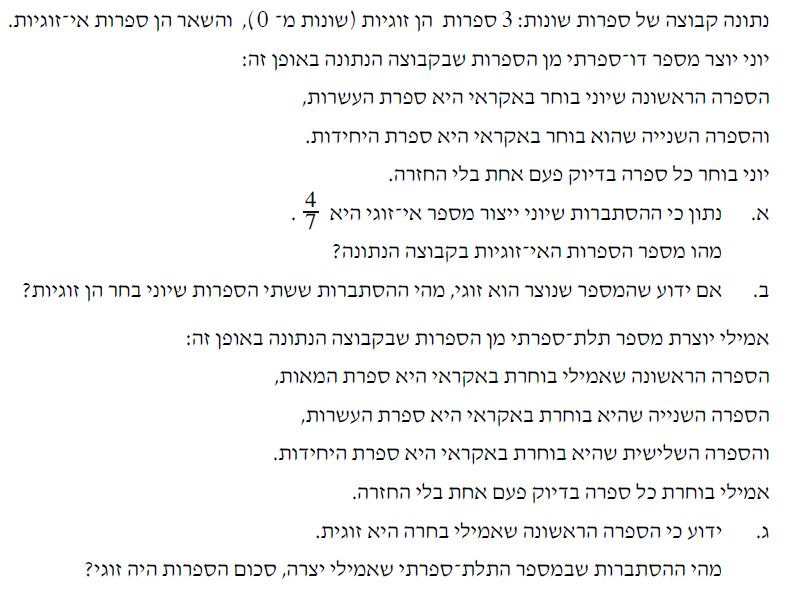
\includegraphics[width=.85\textwidth]{summer-2015a-3}
\end{center}

נסמן 
$=n$
מספר הספרות בקבוצה. מספר הזוגיים 
$3=$,
ומספר האי-זוגיים
$n-3=$.
השאלה מתארת בחירה של "הספרה הראשונה" ואחר כך "הספרה הראשונה", תיאור המכוון לעץ הסתברויות )איור~%
\L{\ref{fig.summer-2015a.1}}(.
כדי לפשט את האיור רשמתי בכל צומת את ההסתברויות ולא את מספר הספרות.

\begin{figure}[H]
\begin{center}
\selectlanguage{english}
\begin{tikzpicture}
[grow=right,
level 1/.append style={text width=2cm,level distance=3.5cm,sibling distance=8em},
level 2/.append style={text width=2.5cm,level distance=4.5cm,sibling distance=4em}]
\node[text width=2cm] {$\left(\frac{3}{n},\frac{n-3}{n}\right)$} % root
child {
  node {$\left(\frac{3}{n-1},\frac{n-4}{n-1}\right)$}
    child {
      node {$\left(\frac{3}{n-2},\frac{n-5}{n-2}\right)\quad *$}
      edge from parent node[below,xshift=5mm,yshift=-1mm] {\R{אי-זוגי}}
    }
    child {
      node {$\left(\frac{2}{n-2},\frac{n-4}{n-2}\right)$}
      edge from parent node[above,xshift=5mm,yshift=1mm] {\R{זוגי}}
    }
    edge from parent node[below,yshift=-1mm] {\R{אי-זוגי}}
}
child { 
  node {$\left(\frac{2}{n-1},\frac{n-3}{n-1}\right)$}
    child {
      node {$\left(\frac{2}{n-2},\frac{n-4}{n-2}\right)\quad *$}
      edge from parent node[below,xshift=5mm,yshift=-1mm] {\R{אי-זוגי}}
    }
    child {
      node {$\left(\frac{1}{n-2},\frac{n-3}{n-2}\right)$}
      edge from parent node[above,xshift=5mm,yshift=1mm] {\R{זוגי}}
    }
    edge from parent node[above] {\R{זוגי}}
};
\end{tikzpicture}
\selectlanguage{hebrew}
\setlength{\belowcaptionskip}{-8ex}
\caption{עץ ההסתברויות של בחירת הספרות}\label{fig.summer-2015a.1}
\end{center}
\end{figure}

\textbf{סעיף א}

המספר יהיה אי-זוגי אם 
\textbf{הבחירה השנייה}
היא של ספרה אי-זוגית. המסלולים האלה מסומנים בכוכביות באיור. נשווה את סכום ההסתברויות של המסלולים לערך הנתון:
\[
\frac{3}{n}\cdot\frac{n-3}{n-1} \;+\; \frac{n-3}{n}\cdot\frac{n-4}{n-1} = \frac{4}{7}\,.
\]
נפשט ונקבל משוואה ריבועית
$n^2-8n+7=0$
שיש לה שני פתרונות לא-שליליים
$n=1,n=7$.
נתון שיש לפחות שלוש ספרות, לכן מספר הספרות הוא
$7$.
שימו לב שהשאלה מבקשת את מספר הספרות 
\textbf{האי-זוגיות}
ולכן התשובה היא
$7-3=4$.

\textbf{סעיף ב}

המילים 
"\textbf{אם ידוע ש-}"
מכוונות להסתברות מותנית. במספר זוגי הספרה האחרונה זוגית:
\vspace{-3ex}
\[
\renewcommand{\arraystretch}{2}
\begin{array}{c}
P(\textrm{\R{שתי ספרות זוגיות}} / \textrm{\R{ספרה אחרונה זוגית}})=\\
\displaystyle\frac{
P(\textrm{\R{שתי ספרות זוגיות}} \cap \textrm{\R{ספרה אחרונה זוגית}})
}
{P(\textrm{\R{ספרה אחרונה זוגית}})}=\\
\displaystyle\frac{
P(\textrm{\R{שתי ספרות זוגיות}})
}
{P(\textrm{\R{ספרה אחרונה זוגית}})}\,.
\end{array}
\]
את החיתוך אפשר לפשט כי אם שתי הספרות זוגיות, הספרה האחרונה חייבת להיות זוגית.

ניתן לחשב את ההסתברות "ספרה אחרונה זוגית" במכנה לפי המידע בעץ ההסתברויות או פשוט לשים לב שהיא המשלימה לערך הנתון בסעיף א של "הספרה האחרונה אי-זוגית". נחשב את ההסתברות במנה לפי המסלול הבודד בעץ ההסתברויות )איור~
\L{\ref{fig.summer-2015a.2}}(
של בחירה של שתי ספרות זוגיות:
\[
\frac{\displaystyle\frac{3}{7}\cdot\frac{2}{6}}{1-\displaystyle\frac{4}{7}}=\frac{1}{3}\,.
\]
\textbf{סעיף ג}

הסכום יהיה זוגי רק אם שתי הספרות האחרונת הן זוגיות או אי-זוגיות:
\begin{eqnarray*}
2k_1+2k_2+2k_3&=&2(k_1+k_2+k_3)\\
2k_1+2(k_2+1)+2(k_3+1)&=&2(k_1+k_2+k_3+1)\,.
\end{eqnarray*}
שני האירועים )בחירת הספרות( בלתי תלויים, ולכן אפשר לבטא את החיתוך כמכפלה:
\vspace{-3ex}
\[
\renewcommand{\arraystretch}{2}
\begin{array}{c}
P(\textrm{\R{סכום זוגי}} / \textrm{\R{ספרה ראשונה זוגית}})=\\
\displaystyle\frac{
P(\textrm{\R{סכום זוגי}} \cap \textrm{\R{ספרה ראשונה זוגית}})
}
{P(\textrm{\R{ספרה ראשונה זוגית}})}=\\
\displaystyle\frac{
P(\textrm{\R{סכום זוגי}}) \cdot P(\textrm{\R{ספרה ראשונה זוגית}})
}
{P(\textrm{\R{ספרה ראשונה זוגית}})}=\\
P(\textrm{\R{סכום זוגי}})\,.
\end{array}
\]
שימו לב שלאחר הבחירה הראשונה של אמילי מספר הספרות הוא שש. לפי עץ ההסתברויות החדש )איור~
\L{\ref{fig.summer-2015a.3}}(
ההסתברות היא:
\[
\frac{2}{6}\cdot\frac{1}{5}+\frac{4}{6}\cdot\frac{3}{5}=\frac{7}{15}\,.
\]

\begin{figure}[H]
\begin{center}
\selectlanguage{english}
\begin{tikzpicture}
[grow=right,
level 1/.append style={level distance=3cm,sibling distance=8em},
level 2/.append style={level distance=4cm,sibling distance=4em}]
\node {$\left(\frac{3}{7},\frac{4}{7}\right)$} % root
child {
  node {$\left(\frac{3}{6},\frac{3}{6}\right)$}
    child {
      node {$\left(\frac{3}{5},\frac{2}{5}\right)$}
      edge from parent node[below,xshift=5mm,yshift=-3mm] {\R{אי-זוגי}}
    }
    child {
      node {$\left(\frac{2}{5},\frac{3}{5}\right)$}
      edge from parent node[above,xshift=5mm,yshift=1mm] {\R{זוגי}}
    }
    edge from parent node[below,yshift=-3mm] {\R{אי-זוגי}}
}
child { 
  node {$\left(\frac{2}{6},\frac{4}{6}\right)$}
    child {
      node {$\left(\frac{2}{5},\frac{3}{5}\right)$}
      edge from parent node[below,xshift=5mm,yshift=-3mm] {\R{אי-זוגי}}
    }
    child {
      node {$\left(\frac{1}{5},\frac{4}{5}\right)\quad$ *}
      edge from parent node[above,xshift=5mm,yshift=1mm] {\R{זוגי} }
    }
    edge from parent node[above,yshift=2mm] {\R{זוגי}}
};
\end{tikzpicture}
\selectlanguage{hebrew}
\caption{עץ ההסתברויות של בחירת הספרות}\label{fig.summer-2015a.2}
\end{center}
\end{figure}
\begin{figure}[H]
\begin{center}
\selectlanguage{english}
\begin{tikzpicture}
[grow=right,
level 1/.append style={level distance=3cm,sibling distance=8em},
level 2/.append style={level distance=4cm,sibling distance=4em}]
\node {$\left(\frac{2}{6},\frac{4}{6}\right)$} % root
child {
  node {$\left(\frac{2}{5},\frac{3}{5}\right)$}
    child {
      node {$\left(\frac{2}{4},\frac{2}{4}\right)$}
      edge from parent node[below,xshift=5mm,yshift=-2mm] {\R{אי-זוגי}}
    }
    child {
      node {$\left(\frac{1}{4},\frac{3}{4}\right)$}
      edge from parent node[above,xshift=5mm,yshift=2mm] {\R{זוגי}}
    }
    edge from parent node[below,yshift=-3mm] {\R{אי-זוגי}}
}
child { 
  node {$\left(\frac{1}{5},\frac{4}{5}\right)$}
    child {
      node {$\left(\frac{1}{4},\frac{3}{4}\right)$}
      edge from parent node[below,xshift=5mm,yshift=-2mm] {\R{אי-זוגי}}
    }
    child {
      node {$\left(\frac{0}{4},\frac{4}{4}\right)\quad$ *}
      edge from parent node[above,xshift=5mm,yshift=2mm] {\R{זוגי}}
    }
    edge from parent node[above,yshift=2mm] {\R{זוגי}}
};
\end{tikzpicture}
\selectlanguage{hebrew}
\caption{עצי ההסתברויות של בחירת הספרות}\label{fig.summer-2015a.3}
\end{center}
\end{figure}
\clearpage

%%%%%%%%%%%%%%%%%%%%%%%%%%%%%%%%%%%%%%%%%%%%%%%%%%%%%%%%%%%%%%%%%%%
\np
\section{חורף תשע"ה}

\begin{center}
\selectlanguage{english}
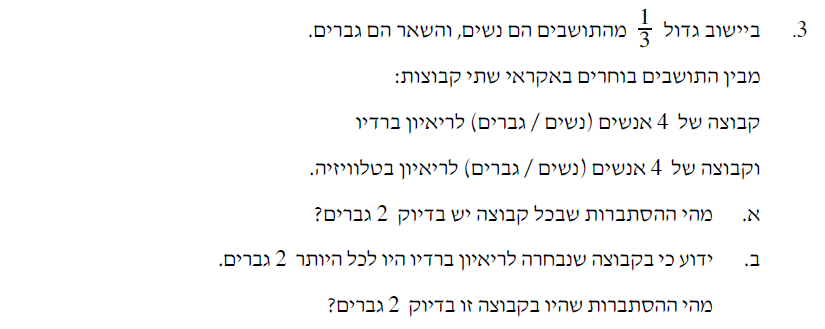
\includegraphics[width=.85\textwidth]{winter-2015-3}
\end{center}

"יישוב גדול" אומר לי שניתן לבחור מספר רב של תושבים, לפחות שמונה תושבים כפי שנדרש.

\textbf{סעיף א}

כל קבוצה היא בחירה בלתי תלוייה:
\[
{4 \choose 2}\left(\frac{2}{3}\right)^2\left(1-\frac{2}{3}\right)^2=\frac{8}{27}\,,
\]
וכדי לקבל את ההסתברות שלשתי הקבוצות יהיו בדיוק שני גברים, נעלה ערך זה בריבוע:
\[
\left(\frac{8}{27}\right)^2=\frac{64}{729}\,.
\]
\textbf{סעיף ב}

המילים
"\textbf{ידוע כי}"
מכוונות להסתברות מותנית:
\vspace{-4ex}
\[
\renewcommand{\arraystretch}{2}
\begin{array}{c}
P(\textrm{\R{בדיוק שני גברים}} / \textrm{\R{לכל היותר שני גברים}})=\\
\displaystyle\frac{
P(\textrm{\R{בדיוק שני גברים}} \cap \textrm{\R{לכל היותר שני גברים}})
}
{P(\textrm{\R{לכל היותר שני גברים}})}\,.
\end{array}
\]
החיתוך במנה שקולה ל-"בדיוק שני גברים" )שחישבנו בסעיף א(, כי "לכל היותר שני גברים" היא 
$0,1,2$
גברים. "לכל היותר שני גברים" הוא הסכום של שלוש נוסחאות ברנולי:
\[
\left(\frac{2}{3}\right)^0\left(\frac{1}{3}\right)^4 + {4\choose 1}\left(\frac{2}{3}\right)^1\left(\frac{1}{3}\right)^3 + {4\choose 2}\left(\frac{2}{3}\right)^2\left(\frac{1}{3}\right)^2=\frac{11}{27}\,
\]
והתשובה לשאלה היא:
\[
\frac{8/27}{11/27}=\frac{8}{11}\,.
\]

%%%%%%%%%%%%%%%%%%%%%%%%%%%%%%%%%%%%%%%%%%%%%%%%%%%%%%%%%%%%%%%%%%%

\np
\section{קיץ תשע"ד מועד ב}

\begin{center}
\selectlanguage{english}
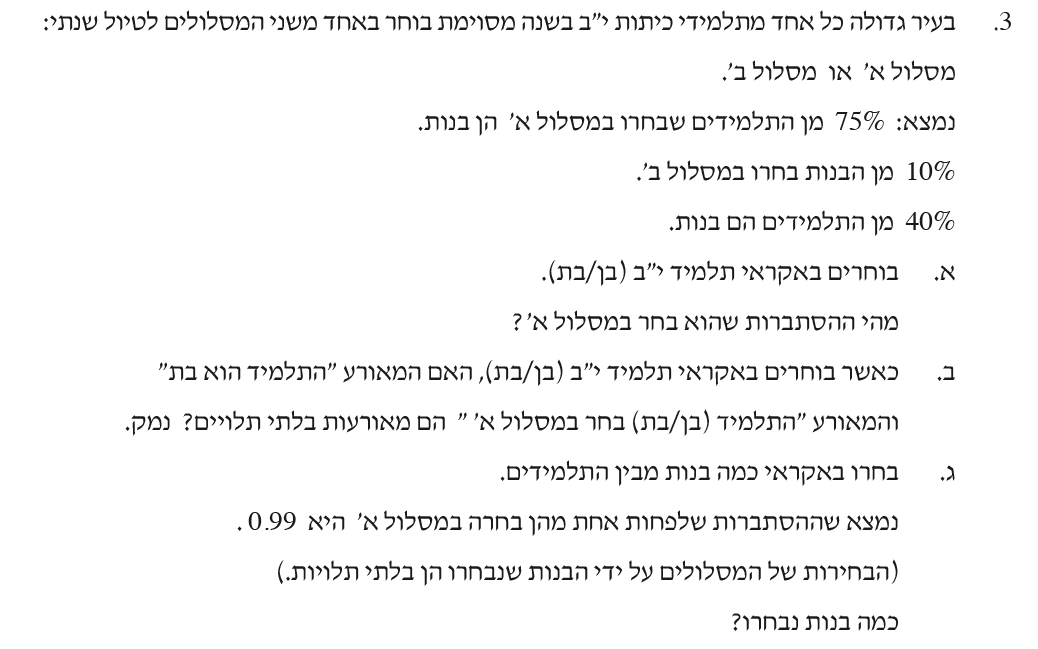
\includegraphics[width=.95\textwidth]{summer-2014b-3}
\end{center}

נמלא את הטבלה ממידע הנתון. נתון ש-% 
$0.4$
מהתלמידים הן בנות. 
$10\%$
מהם בחרו במסלול ב, ולכן נרשום
$0.1\times 0.4=.04$
מעל לתא עם הנתון הראשון. הסתברות המשלימה היא
$0.4-0.04=0.36$.
נתון ש-%
$75\%$
מהתלמידים שבחרו במסלול א הן בנות:
$0.75 \cdot \aleph = 0.36$,
ולכן 
$0.48$
מהתלמידים בחרו מסלול א. ניתן למלא את שאר התאים בטבלה לפי ההסתברויות המשלימות:
\begin{center}
\selectlanguage{english}
\begin{tikzpicture}[scale=2.2]
\draw (0,0) grid (3,3);
\node at (2.5,3.3) {\sffamily\bfseries \R{בנות}};
\node at (1.5,3.3) {\sffamily\bfseries \R{בנים}};
\node at (3.3,2.5) {\sffamily\bfseries \R{א}};
\node at (3.3,1.5) {\sffamily\bfseries \R{ב}};
\node at (2.5,2.7) {$.4-.04=$};
\node at (2.5,2.3) {$.36$};
\node at (0.5,2.7) {$.36/.75=$};
\node at (0.5,2.3) {$.48$};
\node at (1.5,2.7) {$.48-.36=$};
\node at (1.5,2.3) {$.12$};
\node at (0.5,1.7) {$1-.48=$};
\node at (0.5,1.3) {$.52$};
\node at (0.5,0.5) {$1$};
\node at (1.5,0.7) {$1-.4=$};
\node at (1.5,0.3) {$.6$};
\node at (2.5,0.7) {\sffamily\bfseries \R{נתון}};
\node at (2.5,0.3) {$0.4$};
\node at (1.5,1.7) {$.52-.04=$};
\node at (1.5,1.3) {$.48$};
\node at (2.5,1.7) {$.1\times .4=$};
\node at (2.5,1.3) {$.04$};
\end{tikzpicture}
\end{center}
בצורה יותר מפורשת תוך שימוש בהסתברות מותנית:
\[
0.1 = P(\textrm{\R{מסלול ב}} / \textrm{\R{בנות}})=
\displaystyle\frac{
P(\textrm{\R{מסלול ב}} \cap \textrm{\R{בנות}})
}
{P(\textrm{\R{בנות}})}=
\displaystyle\frac{
P(\textrm{\R{מסלול ב}} \cap \textrm{\R{בנות}})
}
{0.4}\,.
\]
מכאן ש:
\[
P(\textrm{\R{מסלול ב}} \cap \textrm{\R{בנות}})
=0.4\cdot 0.1= 0.04\,.
\]
לפי הסתברות משלימה:
\[
P(\textrm{\R{מסלול א}} \cap \textrm{\R{בנות}}) 
= 0.40-0.04=0.36\,.
\]
נמשיך עם הנתון הנוסף:
\[
0.75 = P(\textrm{\R{בנות}} / \textrm{\R{מסלול א}})=
\displaystyle\frac{
P(\textrm{\R{בנות}} \cap \textrm{\R{מסלול א}})
}{P(\textrm{\R{מסלול א}})}=\frac{0.36}{P(\textrm{\R{מסלול א}})}\,.
\]
מכאן ש:
\[
P(\textrm{\R{מסלול א}})=\frac{0.36}{0.75}=0.48\,.
\]
\textbf{סעיף א}

הסעיף מבקש
$P(\textrm{\R{מסלול א}})$
וחישבנו שערכו 
$0.48$.
לכאורה, נראה שמדובר בהסתברות מותנית, אבל מה שידוע הוא שבחרנו 
\textbf{תלמיד כלשהו},
וההסתברות היא אחת.

\textbf{סעיף ב}
\begin{eqnarray*}
P(\textrm{\R{התלמיד הוא בת}} \cap \textrm{\R{מסלול א}}) &=& 
0.36\\
P(\textrm{\R{התלמיד הוא בת}}) \cdot P(\textrm{\R{מסלול א}})
&=&0.4 \cdot 0.48 = 0.192\,.
\end{eqnarray*}
האירועים
\textbf{אינם}
בלתי תלויים.

\textbf{סעיף ג}

כדי לחשב
"\textbf{לפחות אחת}",
נחשב שת ההסתברות המשלימה ל-%
"\textbf{אף אחת}".
ההסתברות שבת לא תבחר מסלול א היא ההסתברות שהיא תבחר מסלול ב:
\[
P(\textrm{\R{מסלול ב}} / \textrm{\R{בת}})=
\displaystyle\frac{
P(\textrm{\R{מסלול ב}} \cap \textrm{\R{בת}})
}{P(\textrm{\R{בת}})}
=\frac{0.04}{0.4}=0.1\,.
\]
נפתור את המשוואה:
\[
(0.1)^n=1-0.99=0.01\,,
\]
ונקבל 
$n=2$.

%%%%%%%%%%%%%%%%%%%%%%%%%%%%%%%%%%%%%%%%%%%%%%%%%%%%%%%%%%%%%%%%%%%
\np
\section{קיץ תשע"ד מועד א}

\begin{center}
\selectlanguage{english}
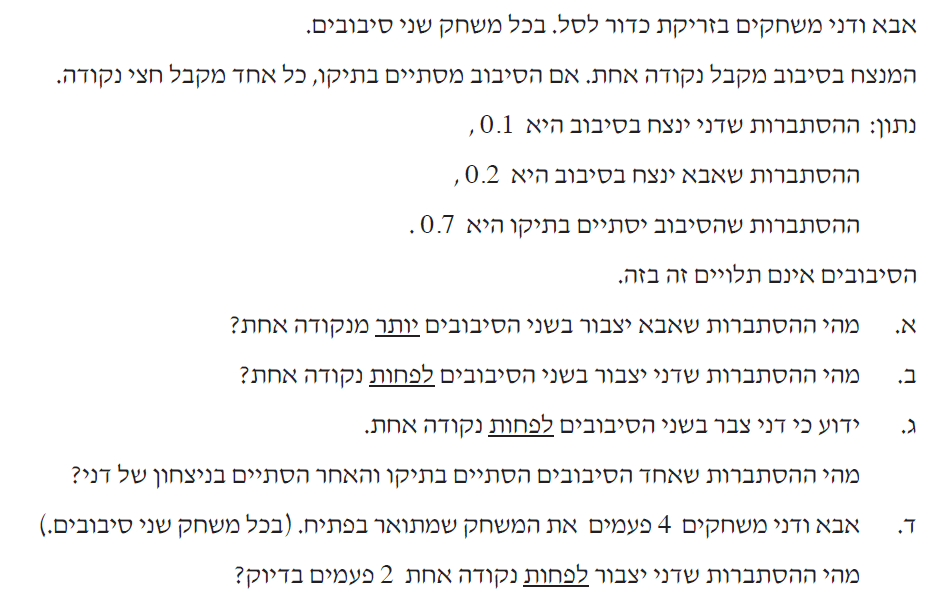
\includegraphics[width=.9\textwidth]{summer-2014a-3}
\end{center}
\vspace{-4ex}

\textbf{סעיף א}

איור~%
\L{\ref{fig.winter-2014.2}}
)למעלה( מראה את צבירת הנקודות של 
\textbf{אבא}
בשני הסיבובים. המצבים בהם אבא צובר
\textbf{יותר}
מנקודה אחת מסומנים בכוכבית. ההסתברות של האירוע היא:
\[
0.2\cdot 0.2 \,+\, 0.2\cdot 0.7 \,+\, 0.7\cdot 0.2 \,=\,0.32\,.
\]
\vspace{-4ex}

\textbf{סעיף ב}

איור~%
\L{\ref{fig.winter-2014.2}}
)למטה( מראה את צבירת הנקודות של
\textbf{דני}
בשני הסיבובים. המצבים בהם דני צובר 
\textbf{לפחות}
נקודה אחת מסומנים בכוכבית. ההסתברות של האירוע היא:
\[
0.2\cdot 0.1 \,+\,0.1\cdot 0.2 \,+\, 0.1\cdot 0.1 \,+\,0.1\cdot 0.7 \,+\, 0.7\cdot 0.1\,+\,0.7\cdot 0.7\,=\,0.68\,.
\]
\vspace{-4ex}

\textbf{סעיף ג}

המילים
"\textbf{ידוע כי}"
מכוונות להסתברות מותנית והחיתוך מצטמצם כי אם יש תיקו אחד וניצחון של דני אז דני צבר לפחות נקודה אחת:
\vspace{-2ex}
\[
\renewcommand{\arraystretch}{2}
\begin{array}{c}
P(\textrm{\R{תיקו אחד, ניצחון אחד לדני}} / \textrm{\R{דני צבר לפחות נקודה אחת}})=\\
\displaystyle\frac{
P(\textrm{\R{תיקו אחד, ניצחון אחד לדני}} \cap \textrm{\R{דני צבר לפחות נקודה אחת}})
}
{P(\textrm{\R{דני צבר לפחות נקודה אחת}})}=\\
\displaystyle\frac{
P(\textrm{\R{תיקו אחד, ניצחון אחד לדני}})
}
{P(\textrm{\R{דני צבר לפחות נקודה אחת}})}\,.
\end{array}
\]
נחשב את המנה על ידי חיבור ההסתברויות של שני מסלולים בעץ המסומנים ב-%
$\#$:
\[
\frac{0.1\cdot 0.7 \,+\, 0.7\cdot 0.1}{0.68} = .2059\,.
\]
\textbf{סעיף ד}

סעיף ב חישבנו את ההסתברות של האירוע בכל סיבוב, ונשאר רק לחשב:
\vspace{-1ex}
\[
{4\choose 2}(0.68)^2 (0.32)^2= 0.2841\,.
\]
\vspace{-2ex}
\begin{figure}[H]
\begin{center}
\selectlanguage{english}
\begin{tikzpicture}
[align=left,grow=right,
level 1/.append style={font=\sffamily,level distance=3cm,sibling distance=8em},
level 2/.append style={font=\sffamily,level distance=4cm,sibling distance=3em}]
\node[left] {$0$} % root
child {
  node[right] {$\frac{1}{2}$}
    child {
      node[right] {$1$}
      edge from parent node[below,yshift=-1mm] {$0.7$}
    }
    child {
      node[right] {$\frac{1}{2}$}
      edge from parent node[below,xshift=4mm] {$0.1$}
    }
    child {
      node[right] {$1\frac{1}{2}\quad *$}
      edge from parent node[above,yshift=1mm] {$0.2$}
    }
    edge from parent node[below,xshift=-4mm,yshift=-3mm] {\R{תיקו}
$0.7$}
}
child {
  node[right] {$0$}
    child {
      node[right] {$\frac{1}{2}$}
      edge from parent node[below,yshift=-1mm] {$0.7$}
    }
    child {
      node[right] {$0$}
      edge from parent node[below,xshift=4mm] {$0.1$}
    }
    child {
      node[right] {$1$}
      edge from parent node[above,yshift=1mm] {$0.2$}
    }
    edge from parent node[below] {\R{דני}
$0.1$}
}
child {
  node[right] {$1$}
    child {
      node[right] {$1\frac{1}{2}\quad *$}
      edge from parent node[below,yshift=-1mm] {$0.7$}
    }
    child {
      node[right] {$1$}
      edge from parent node[below,xshift=4mm] {$0.1$}
    }
    child {
      node[right] {$2\quad *$}
      edge from parent node[above,yshift=1mm] {$0.2$}
    }
    edge from parent node[above,xshift=-4mm,yshift=3mm] {\R{אבא}
$0.2$}
};
\end{tikzpicture}
\smallskip
\begin{tikzpicture}
[grow=right,
level 1/.append style={font=\sffamily,level distance=3cm,sibling distance=8em},
level 2/.append style={font=\sffamily,level distance=4cm,sibling distance=3em}]
\node[left] {$0$} % root
child {
  node[right] {$\frac{1}{2}$}
    child {
      node[right] {$1\quad *$}
      edge from parent node[below,yshift=-1mm] {$0.7$}
    }
    child {
      node[right] {$1\frac{1}{2}\quad *\quad \#$}
      edge from parent node[below,xshift=4mm] {$0.1$}
    }
    child {
      node[right] {$\frac{1}{2}$}
      edge from parent node[above,yshift=1mm] {$0.2$}
    }
    edge from parent node[below,xshift=-4mm,yshift=-3mm] {\R{תיקו}
$0.7$}
}
child {
  node[right] {$1$}
    child {
      node[right] {$1\frac{1}{2}\quad *\quad \#$}
      edge from parent node[below,yshift=-1mm] {$0.7$}
    }
    child {
      node[right] {$2\quad *$}
      edge from parent node[below,xshift=4mm] {$0.1$}
    }
    child {
      node[right] {$1\quad *$}
      edge from parent node[above,yshift=1mm] {$0.2$}
    }
    edge from parent node[below] {\R{דני}
$0.1$}
}
child {
  node[right] {$0$}
    child {
      node[right] {$\frac{1}{2}$}
      edge from parent node[below,yshift=-1mm] {$0.7$}
    }
    child {
      node[right] {$1\quad *$}
      edge from parent node[below,xshift=4mm] {$0.1$}
    }
    child {
      node[right] {$0$}
      edge from parent node[above,yshift=1mm] {$0.2$}
    }
    edge from parent node[above,xshift=-4mm,yshift=3mm] {\R{אבא}
$0.2$}
};
\end{tikzpicture}
\selectlanguage{hebrew}
\setlength{\belowcaptionskip}{-4ex}
\caption{עץ ההסתברויות של צבירת נקודות של אבא )למעלה( ודני )למטה(}\label{fig.winter-2014.2}
\end{center}
\end{figure}


%%%%%%%%%%%%%%%%%%%%%%%%%%%%%%%%%%%%%%%%%%%%%%%%%%%%%%%%%%%%%%%%%%%
\np
\section{חורף תשע"ד}

\begin{center}
\selectlanguage{english}
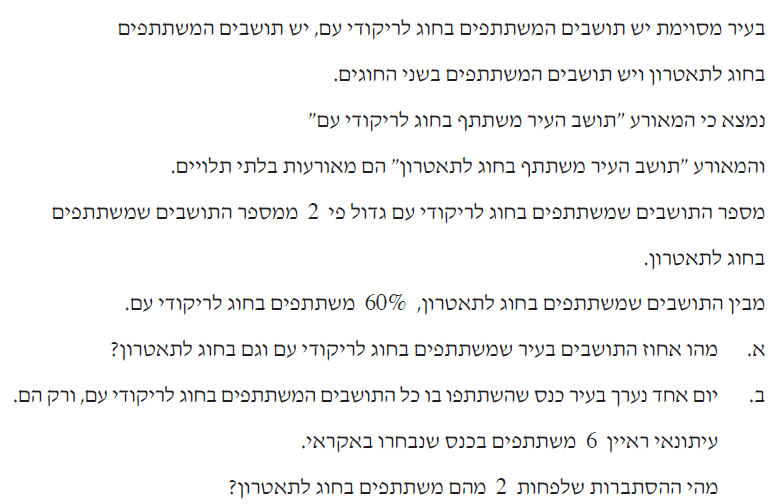
\includegraphics[width=.9\textwidth]{winter-2014-3}
\end{center}

נסמן
$=T$
מספר המשתתפים בתאטרון,
$=R$
מספר המשתתפים בריקודי עם. המילה 
"\textbf{מבין}"
מכוונת להתסברות מותנית. נתון
$P(R/T)=0.6$
וגם שהאירועים בלתי תלויים. נחשב:
\[
0.6=P(R/T)=\frac{P(R\cap T)}{P(T)}=\frac{P(R)\cdot P(T))}{P(T)}=P(R)\,.
\]
ביחד עם הנתון
$P(R)=2P(T)$
נתחיל למלא את הטבלה:
\begin{center}
\selectlanguage{english}
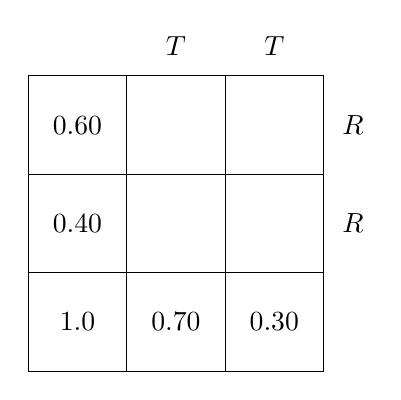
\begin{tikzpicture}[scale=1.25]
\draw (0,0) grid (3,3);
\node at (2.5,3.3) {$\bm{T}$};
\node at (1.5,3.3) {$\bover{T}$};
\node at (3.3,2.5) {$\bm{R}$};
\node at (3.3,1.5) {$\bover{R}$};
\node at (0.5,2.5) {$0.60$};
\node at (2.5,0.5) {$0.30$};
\node at (.5,.5) {$1.0$};
\node at (1.5,.5) {$0.70$};
\node at (.5,1.5) {$0.40$};
\end{tikzpicture}
\end{center}
שוב נסתמך על העובדה שהאירועים בלתי תלויים ונקבל:
\[
P(R\cap T)=P(R)\cdot P(T)=0.6\cdot 0.3=0.18\,,
\]
ואז יש לנו מספיק נתונים למלא את הטבלה:
\begin{center}
\selectlanguage{english}
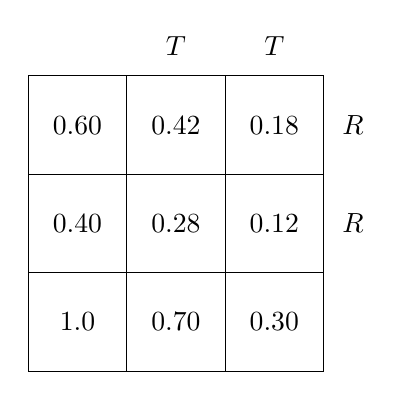
\begin{tikzpicture}[scale=1.25]
\draw (0,0) grid (3,3);
\node at (2.5,3.3) {$\bm{T}$};
\node at (1.5,3.3) {$\bover{T}$};
\node at (3.3,2.5) {$\bm{R}$};
\node at (3.3,1.5) {$\bover{R}$};
\node at (2.5,2.5) {$0.18$};
\node at (0.5,2.5) {$0.60$};
\node at (1.5,2.5) {$0.42$};
\node at (0.5,1.5) {$0.40$};
\node at (0.5,0.5) {$1.0$};
\node at (1.5,0.5) {$0.70$};
\node at (2.5,0.5) {$0.30$};
\node at (1.5,1.5) {$0.28$};
\node at (2.5,1.5) {$0.12$};
\end{tikzpicture}
\end{center}
\textbf{סעיף א}

חישבנו ש-%
$P(R\cap T)=0.18$.

\textbf{סעיף ב}

המילים "כל התושבים המשתתפים בחוג לריקודי עם,
\textbf{ורק הם}"
מכוונות להסתברות מותנית. אם ידוע שתושב משתתף בריקודי עם, ההסתברות שהוא משתתף גם בתאטרון היא:
\[
P(T/R) = \frac{P(T\cap R)}{P(R)}= \frac{0.18}{.060} = 0.3\,.
\]
כדי לחשב "לפחות שניים" עדיף לחשב את המשלים ל-"אפס או אחד":
\[
1-{6\choose 0}(0.3)^0(0.7)^6 -{6\choose 1}(0.3)^1(0.7)^5=0.5798\,.
\]

%%%%%%%%%%%%%%%%%%%%%%%%%%%%%%%%%%%%%%%%%%%%%%%%%%%%%%%%%%%%%%%%%%%

\np
\section{המלצות}

\begin{itemize}
\item
\textbf{קרא בזהירות את השאלה}. 
לעתים השאלות ארוכות )בחינות של קיץ תשע"ה א, קיץ תשע"ח ב( וחשוב להבין את המשמעות של כל פסקה.

%%%%%%%%%%%%%%%%%%%%%%%%%%%%%%%%%%%%

\item
כמעט כל הבחינות מכילות שאלות על 
\textbf{הסתברות מותנית}.
ניסוחים רבים מכוונים להסתברות מותנית וחשוב להכיר אותם!

\begin{itemize}
\item
הניסוח השכיח ביותר משתמש במילים
"\textbf{אם ידוע ש-}"
או
"\textbf{ידוע כי}".

\item
בבחינה של חורף תשע"ז
כתוב "%
\textbf{אם} $\ldots$ ,
\textbf{מהי ההסתברות} $\ldots$".
לא לגמרי ברור שלמילה "אם" יש משמעות של "אם ידוע", אבל זאת הכוונה.

\item
לעתים קרובות )למשל, בבחינה של קיץ תשע"ה ב( כתוב "%
\textbf{מה ההסתברות לבחור} $\ldots$
\textbf{מבין} $\ldots$".

\item
יוצא מן הכלל: בבחינה של קיץ תשע"ו א כתוב
"\textbf{מבין}
כל הנבחנים" והמילה "מבין" בדרך כלל מכוונת להסתברות מותנית, אבל כאשר "מבין" מתייחס ל-%
"\textbf{כל}
הנבחנים" אין הסתברות מותנית, או ההסתברות מותנית בהסתברות שהיא 
$1$,
והחיתוך מצטמצם:
\[
P(X/\textrm{\R{כל הנבחנים}})=
\frac{P(X\cap \textrm{\R{כל הנבחנים}})}
{P(\textrm{\R{כל הנבחנים}})} = 
\frac{P(X)}{1}=P(X)\,.
\]
מצב דומה מופיע בבחינה של קיץ תשע"ד ב )"בוחרים באקראי תלמיד י"ב )בן/בת("(, ובבחינה של קיץ תשע"ח ב )"מן התלמידים שנגשו למבחן"(.

\item
בבחינה של קיץ תשע"ח א הניסוח הוא: "%
$\ldots X\%$
נעזרו 
$\ldots$.
$\displaystyle\frac{k}{n}$
\textbf{מהם}
עברו את הבחינה".

\item
בבחינה של חורף תשע"ד יש ניסוח אחר:
\textbf{כל התושבים המשתתפים ב-} $\ldots$,
\textbf{ורק הם}.
\end{itemize}

%%%%%%%%%%%%%%%%%%%%%%%%%%%%%%%%%%%%

\item
כאשר יש חיתוך בחישוב של הסתברות מותנית, לעתים קרובות ניתן לפשט את החישוב. בבחינה של קיץ תשע"ז א יש לחשב
$P(D=4\cap D\ge 3)$,
אבל אם ערך גדול או שווה
$3$
\textbf{וגם}
שווה ל-%
$4$,
אז הוא שווה ל-%
$4$, 
ולכן מספיק לחשב
$P(D=4)$.

%%%%%%%%%%%%%%%%%%%%%%%%%%%%%%%%%%%%

\item
כאשר יש חיתוך בין שני אירועים בלתי תלויים, חישוב ההסתברות המותנית מצטמצם )בחינה של קיץ תשע"ה א(:
\[
\renewcommand{\arraystretch}{2.4}
\begin{array}{l}
\displaystyle\frac{
P(\textrm{\R{סכום זוגי}} \cap \textrm{\R{ספרה ראשונה זוגית}})
}{P(\textrm{\R{ספרה ראשונה זוגית}})}=\\
\displaystyle\frac{
P(\textrm{\R{סכום זוגי}}) \cdot P(\textrm{\R{ספרה ראשונה זוגית}})
}
{P(\textrm{\R{ספרה ראשונה זוגית}})}=\\
P(\textrm{\R{סכום זוגי}})
\,.
\end{array}
\]
מצב דומה מופיע בבחינות של חורף תשע"ז וחורף משע"ח.
%%%%%%%%%%%%%%%%%%%%%%%%%%%%%%%%%%%%

\item
בבחינה של חורף תשע"ד נתון
$P(T/R)$
וגם נתון ששני אירועים הם
\textbf{בלתי תלויים}.
החיתוך שווה למכפלת ההסתברויות והחישוב מצטמצם:
\[
P(T/R) = \frac{P(T \cap R)}{P(R)} =\frac{P(T)\cdot P(R)}{P(R)} = P(T)\,.
\]
\vspace{-4ex}
%%%%%%%%%%%%%%%%%%%%%%%%%%%%%%%%%%%%

\item
המילה 
\textbf{בדיוק}
מכוונת לחישוב אחד של נוסחת ברנולי, כי נתון כמה "הצלחות" צריכות להיות וגם כמה "כשלונות". מקרה מעניין נמצא בבחינה של קיץ תשע"ח ב כאשר נתון שההסתברות לקבל 
$60$
שווה להסתברות לקבל
$100$.
נתון גם שיש שלוש הצלחות מתוך חמש )%
$20$
נקודות כל אחת(, אז ההסתברות לקבל שני כשלונות )%
$20$
נקודות כל אחת( צריכה להיות שווה להסתברות לקבל שתי הצלחות )%
$20$
נקודות כל אחת(.

%%%%%%%%%%%%%%%%%%%%%%%%%%%%%%%%%%%%

\item
בבחינה של קיץ תשע"ז א כתוב "%
\textbf{בוחרים באקראי}
$\ldots$,
\textbf{עד של-}
$3$
מהם
\textbf{בדיוק}
יש קלנועית". המשמעות של "עד ש-" היא שמפסיקים את הבחירה האקראית כאשר הבחירה 
\textbf{האחרונה} 
היא "הצלחה". במקרה זה נשארו שתי "הצלחות" שיש לחשב את ההסתברות שלהן לפי נוסחת ברנולי, ואז להכפיל בהסתברות של "הצלחה" בבחירה האחרונה:
\[
\overbrace{\pm\;\pm\;\pm\;\pm\;\pm}^{2/5}\quad\quad \overbrace{+}^{1/1}\,.
\]
\vspace{-6ex}
%%%%%%%%%%%%%%%%%%%%%%%%%%%%%%%%%%%%

\item
בבחינה של קיץ תשע"ז ב הביטוי "מוציאים באקראי
$\ldots$",
ובהמשך הביטוי "מוציאים באקראי
\textbf{שוב}
$\ldots$"
מכוון לשימוש בעץ כדי לתאר את הבחירה הסדרתית.

%%%%%%%%%%%%%%%%%%%%%%%%%%%%%%%%%%%%

\item
בבחינה של קיץ תשע"ח א, המשמעות של הניסוח "%
\textbf{לפחות אחת}
משתי הטענות 
$I, II$"
היא שהאירוע קורה אם קורה אחד מהאירועים
$I, II$,
\textbf{או שניהם},
המסומן 
$I \cup II$.
יש שתי דרכים לחשב את ההסתברות: על ידי חיבור ההסתברות של שני האירועים וחיסור האירוע המשותף כדי לקזז את הספירה הכפולה, או לחבר את האירוע המשותף עם האירועים של אחד ולא השני המסומן 
$I-II, II-I$:
\begin{eqnarray*}
P(I \cup II) &=& P(I) + P(II) - P(I \cap II)\\
P(I \cup II) &=& P(I-II) + P(II-I) + P(I \cap II)\,.
\end{eqnarray*}
הערכים לחישוב
$P(I \cup II)$
בשתי הדרכים מסומנים בטבלה להלן, כאשר התא המקווקו מופיע פעמיים, פעם כחלק מהאירוע
$I$
ופעם כחלק מהאירוע
$II$:
\begin{center}
\selectlanguage{english}
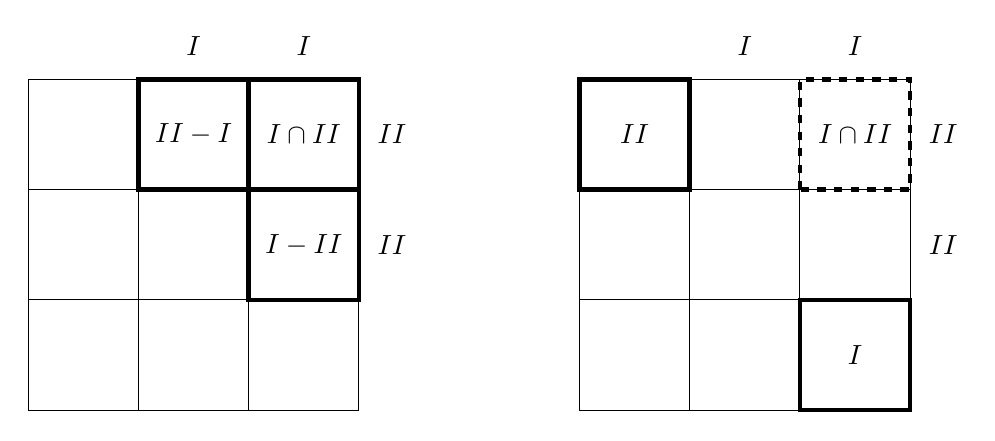
\begin{tikzpicture}[scale=1.4]
\begin{scope}
\draw (0,0) grid (3,3);
\node at (2.5,3.3) {$\bm{I}$};
\node at (1.5,3.3) {$\bover{I}$};
\node at (3.3,2.5) {$\bm{II}$};
\node at (3.3,1.5) {$\bover{II}$};
\node at (2.5,2.5) {$I\cap II$};
\node at (2.5,1.5) {$I-II$};
\node at (1.5,2.5) {$II-I$};
\draw[ultra thick] (2,2) rectangle +(1,1);
\draw[ultra thick] (1,2) rectangle +(1,1);
\draw[ultra thick] (2,1) rectangle +(1,1);
\end{scope}
\begin{scope}[xshift=5cm]
\draw (0,0) grid (3,3);
\node at (2.5,3.3) {$\bm{I}$};
\node at (1.5,3.3) {$\bover{I}$};
\node at (3.3,2.5) {$\bm{II}$};
\node at (3.3,1.5) {$\bover{II}$};
\node at (2.5,2.5) {$I\cap II$};
\node at (2.5,0.5) {$I$};
\node at (0.5,2.5) {$II$};
\draw[ultra thick] (0,2) rectangle +(1,1);
\draw[ultra thick] (2,0) rectangle +(1,1);
\draw[ultra thick,dashed] (2,2) rectangle +(1,1);
\end{scope}
\end{tikzpicture}
\end{center}

%%%%%%%%%%%%%%%%%%%%%%%%%%%%%%%%%%%%

\item
בבחינה של חורף תשע"ו נתון ההסתברות
$p$
ש-"לא יזכה
\textbf{באף משחק}
מתוך 
$n$
משחקים". גם בבחינה של  קיץ תשע"ח ב צריכים לחשב את ההסבתרות של תשובה נכונה 
\textbf{לכל}
השאלות או תשובה נכונה
\textbf{לאף אחת}
מהשאלות.  אין צורך להשתמש בנוסחת ברנולי במלואו:
\[
{n \choose k}p^k(1-p)^{n-k}\,.
\]
אם
$k=0$
או
$k=n$,
${n\choose k}=1$.
גם
$p^n(1-p)^0=p^n\cdot 1$
או
$p^0(1-p)^n=1\cdot(1-p)^n$,
ונשאר רק גורם אחד 
$p^n$
או
$(1-p)^n$.

%%%%%%%%%%%%%%%%%%%%%%%%%%%%%%%%%%%%

\item
בבחינות של קיץ תשע"ו א, ב יש שלוש תוצאות אפשרויות במקום שתיים. סכום ההסתברויות חייב להיות אחד, ולכן כאשר מחשבים משלים להסתברות אחת, יש להחסיר את שתי ההסתברויות האחרות. בבחינה של מועד ב, ההסתברות לתיקו היא אחד פחות ההסתברות שיעל תנצח פחות ההסתברות אנה תנצח:
\[
P(\textrm{\R{תיקו}}) =
1 - (P(\textrm{\R{יעל}})+
P(\textrm{\R{אנה}})) = 
1 - P(\textrm{\R{יעל}})-
P(\textrm{\R{אנה}}) \,.
\]
\vspace{-4ex}
\item 
במספר בחינות )חורף תשע"ה, קיץ תשע"ד ב, קיץ תשע"ה ב( כתוב "ישוב גדול", "עיר גדולה", "אוניברסיטה גדולה". אני מניח שבמילה "גדול" מבטיחה שאפשר לבחור תושבים או סטודנטים כפי שדרוש  בשאלות. אין משמעות לבחור ארבעה סטודנטים אם יש רק שניים באוניברסיטה.
\end{itemize}

